% !TEX program = xelatex
% !TEX encoding = UTF-8 Unicode
% Seminar: Probleme de examen - exemple rezolvate din anii precedenți
% Statistica Piețelor Financiare
% Surse: Probleme examen 2020, 2021, 2022 (restanță 2), 2024
%
% IMPORTANT: Acest document folosește fontspec/polyglossia (diacritice românești).
%            Compilați NUMAI cu xelatex (sau lualatex), NU cu pdflatex.
%
% Compilare:
%   xelatex seminar_probleme_examen_ro.tex
%   xelatex seminar_probleme_examen_ro.tex   (rerun pentru toc / ref)

\documentclass[9pt, aspectratio=169, t]{beamer}
%=============================================================================
% PREAMBUL COMUN - Statistica Piețelor Financiare
% Versiune robustă pentru macOS (MacTeX / BasicTeX / TeX Live)
% Daniel Traian Pele, Antoaneta Amza - ASE București
%
% MODIFICĂRI față de varianta originală:
%  (1) fontawesome5 făcut OPȚIONAL (\IfFileExists) → nu mai pică dacă lipsește
%  (2) polyglossia cu fallback automat pe babel dacă romanian nu există
%  (3) setmainfont rescris cu Ligatures=TeX și nume normalizate (merge pe macOS)
%  (4) graphicspath extins (include directorul curent + variante relative) ca
%      logo-urile să fie găsite și când lansezi xelatex dintr-un subdirector
%
% Compilare:  xelatex preamble + main, de DOUĂ ori (toc/ref).
%=============================================================================

% Asigură încadrarea conținutului pe diapozitive
\setbeamersize{text margin left=8mm, text margin right=8mm}

%=============================================================================
% CONFIGURARE TEMĂ ȘI STIL
%=============================================================================
\usetheme{default}

% Paletă de Culori
\definecolor{MainBlue}{RGB}{26, 58, 110}
\definecolor{AccentBlue}{RGB}{26, 58, 110}
\definecolor{IDAred}{RGB}{205, 0, 0}
\definecolor{DarkGray}{RGB}{51, 51, 51}
\definecolor{MediumGray}{RGB}{128, 128, 128}
\definecolor{LightGray}{RGB}{248, 248, 248}
\definecolor{VeryLightGray}{RGB}{235, 235, 235}
\definecolor{KeynoteGray}{RGB}{218, 218, 218}
\definecolor{SectionGray}{RGB}{120, 120, 120}
\definecolor{FooterGray}{RGB}{100, 100, 100}
\definecolor{Crimson}{RGB}{220, 53, 69}
\definecolor{Forest}{RGB}{46, 125, 50}
\definecolor{Amber}{RGB}{181, 133, 63}
\definecolor{Orange}{RGB}{230, 126, 34}
\definecolor{Purple}{RGB}{142, 68, 173}

% Fundal gradient (gradient Keynote exact 315°: alb la RGB 218,218,218)
\setbeamertemplate{background}{%
	\begin{tikzpicture}[remember picture, overlay]
		\shade[shading=axis, shading angle=315,
		top color=white, bottom color=KeynoteGray]
		(current page.south west) rectangle (current page.north east);
	\end{tikzpicture}%
}
% Culoare solidă de rezervă pentru compatibilitate
\setbeamercolor{background canvas}{bg=}

\setbeamercolor{palette primary}{bg=MainBlue, fg=white}
\setbeamercolor{palette secondary}{bg=MainBlue!85, fg=white}
\setbeamercolor{palette tertiary}{bg=MainBlue!70, fg=white}
\setbeamercolor{structure}{fg=MainBlue}
\setbeamercolor{title}{fg=IDAred}
\setbeamercolor{frametitle}{fg=IDAred, bg=}
\setbeamercolor{block title}{bg=MainBlue, fg=white}
\setbeamercolor{block body}{bg=VeryLightGray, fg=DarkGray}
\setbeamercolor{block title alerted}{bg=Crimson, fg=white}
\setbeamercolor{block body alerted}{bg=Crimson!8, fg=DarkGray}
\setbeamercolor{block title example}{bg=Forest, fg=white}
\setbeamercolor{block body example}{bg=Forest!8, fg=DarkGray}
\setbeamercolor{item}{fg=MainBlue}

\setbeamerfont{institute}{size=\footnotesize}

\setbeamercolor{author in head/foot}{fg=FooterGray, bg=}
\setbeamercolor{title in head/foot}{fg=FooterGray, bg=}
\setbeamercolor{date in head/foot}{fg=FooterGray, bg=}
\setbeamercolor{section in head/foot}{fg=FooterGray, bg=}
\setbeamercolor{subsection in head/foot}{fg=FooterGray, bg=}

\setbeamertemplate{itemize item}{\color{MainBlue}$\boxdot$}
\setbeamertemplate{itemize subitem}{\color{MainBlue}$\blacktriangleright$}
\setbeamertemplate{itemize subsubitem}{\color{MainBlue}\tiny$\bullet$}
\setbeamertemplate{itemize/enumerate body begin}{\normalsize}
\setbeamertemplate{itemize/enumerate subbody begin}{\normalsize}

\setbeamertemplate{section in toc}{%
	\leavevmode\leftskip=1.5em%
	\llap{\color{MainBlue}$\boxdot$\kern0.5em}%
	\inserttocsection\par%
}

\setlength{\leftmargini}{10pt}
\setlength{\leftmarginii}{10pt}
\makeatletter
\def\@listi{\leftmargin\leftmargini \topsep 0pt \parsep 0pt \itemsep 0pt}
\def\@listii{\leftmargin\leftmarginii \topsep 0pt \parsep 0pt \itemsep 0pt}
\makeatother

\setbeamertemplate{navigation symbols}{}

%=============================================================================
% ANTET PERSONALIZAT
%=============================================================================
\setbeamertemplate{headline}{%
	\vskip10pt%
	\hbox to \paperwidth{%
		\hskip0.5cm%
		{\small\color{FooterGray}\renewcommand{\hyperlink}[2]{##2}\insertsectionhead}%
		\hfill%
		\textcolor{FooterGray}{\small\insertframenumber}%
		\hskip0.5cm%
	}%
	\vskip4pt%
	{\color{FooterGray}\hrule height 0.4pt}%
}

%=============================================================================
% PACHETE — ordine importantă: fontspec ÎNAINTE de polyglossia/babel
%=============================================================================

% --- (1) FONTSPEC + FONTURI ROBUSTE PE macOS ---
\usepackage{fontspec}
% Pe macOS unele fonturi Latin Modern nu sunt înregistrate ca fonturi de sistem.
% Folosim Ligatures=TeX (pentru -- → en-dash etc.) și lăsăm fontspec să caute
% prin kpathsea (merge atât pe Mac, cât și pe Linux/Windows).
\defaultfontfeatures{Ligatures=TeX}
\IfFontExistsTF{Latin Modern Roman}{%
	\setmainfont{Latin Modern Roman}
	\setsansfont{Latin Modern Sans}
	\setmonofont{Latin Modern Mono}
}{%
	% Fallback dacă numele cu spații nu sunt găsite (cazul macOS fără fonturi
	% Latin Modern în /Library/Fonts) — fontspec va folosi fontul implicit.
	\PackageWarning{preamble}{Latin Modern Roman nu a fost gasit; folosesc fontul implicit.}
}

% --- (2) POLYGLOSSIA SAU BABEL CU FALLBACK ---
% Pe versiuni vechi de polyglossia (TeX Live < 2020) limba `romanian` nu există.
% Detectăm și folosim babel ca rezervă.
\IfFileExists{gloss-romanian.ldf}{%
	\usepackage{polyglossia}
	\setdefaultlanguage{romanian}
	\setotherlanguage{english}
}{%
	\PackageWarning{preamble}{polyglossia/romanian indisponibil; folosesc babel.}
	\usepackage[english,romanian]{babel}
}

% --- (3) MATH ȘI GRAFICĂ ---
\usepackage{amsmath, amssymb, amsthm}
\usepackage{mathtools}
\usepackage{bm}
\usepackage{tikz}
\usetikzlibrary{arrows.meta, positioning, shapes, calc, decorations.pathreplacing, shadings}
\usepackage{booktabs}
\usepackage{multirow}
\usepackage{array}
\usepackage{graphicx}
\usepackage{hyperref}
\usepackage{colortbl}
\usepackage{listings}
\lstset{basicstyle=\ttfamily\small, breaklines=true, frame=single, backgroundcolor=\color{VeryLightGray}}
\hypersetup{colorlinks=true, linkcolor=MainBlue, urlcolor=MainBlue}

% --- (4) GRAPHICSPATH cu directorul curent inclus ca fallback ---
\graphicspath{{./}{./logos/}{./charts/}{./photos/}{../logos/}{../charts/}{../photos/}{../../logos/}{../../charts/}{../../photos/}}
\hfuzz=2pt
\vfuzz=2pt

%=============================================================================
% SUBSOL PERSONALIZAT — fontawesome5 făcut OPȚIONAL
%=============================================================================
% Pe BasicTeX / instalări minime de MacTeX, fontawesome5 nu există.
% Dacă lipsește, omitem icoanele (subsolul rămâne curat).
\IfFileExists{fontawesome5.sty}{%
	\usepackage{fontawesome5}
	\newcommand{\hasfontawesome}{true}
}{%
	\PackageWarning{preamble}{fontawesome5 indisponibil; subsolul nu va contine icoane.}
}

\setbeamertemplate{footline}{%
	{\color{FooterGray}\hrule height 0.4pt}%
	\vskip4pt%
	\hbox to \paperwidth{%
		\hskip0.5cm%
		\textcolor{FooterGray}{\small Statistica Piețelor Financiare}%
		\hfill%
		\raisebox{-0.1em}{%
			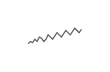
\begin{tikzpicture}[x=0.08em, y=0.08em, line width=0.4pt]
				\draw[FooterGray] (0,3) -- (1,4) -- (2,3.5) -- (3,5) -- (4,4) -- (5,6) -- (6,5.5) -- (7,4) -- (8,5) -- (9,7) -- (10,6) -- (11,5) -- (12,6.5) -- (13,8) -- (14,7) -- (15,6) -- (16,7.5) -- (17,9) -- (18,8) -- (19,7) -- (20,8.5) -- (21,10) -- (22,9) -- (23,8) -- (24,9.5);
			\end{tikzpicture}%
		}%
		\hskip0.5cm%
	}%
	\vskip6pt%
}

%=============================================================================
% COMANDA QUANTLET
%=============================================================================
\newcommand{\quantlet}[2]{%
	\hfill\href{#2}{%
		\raisebox{-0.15em}{
\includegraphics[height=0.7em]{ql_logo.png}}%
		\textcolor{MainBlue}{\tiny\ #1}%
	}%
}

%=============================================================================
% PAGINĂ TITLU PERSONALIZATĂ
%=============================================================================
\defbeamertemplate*{title page}{hybrid}[1][]
{
	\vspace{0.2cm}
	\noindent\makebox[\linewidth][s]{%
		\href{https://www.ase.ro}{
\includegraphics[height=1.0cm]{ase_logo.png}}\hfill%
		\href{https://theida.net}{
\includegraphics[height=1.0cm]{ida_logo.png}}\hfill%
		\href{https://blockchain-research-center.com}{
\includegraphics[height=1.0cm]{brc_logo.png}}\hfill%
		\href{https://www.ai4efin.ase.ro}{
\includegraphics[height=1.0cm]{ai4efin_logo.png}}\hfill%
		\href{https://ipe.ro/new}{
\includegraphics[height=1.0cm]{acad_logo.png}}\hfill%
		\href{https://www.digital-finance-msca.com}{
\includegraphics[height=1.0cm]{msca_logo.png}}%
	}
	\vspace{0.6cm}
	
	\noindent\makebox[\linewidth][c]{%
		\begin{minipage}{0.11\linewidth}
			\centering
			\href{https://quantlet.com}{
\includegraphics[height=1.1cm]{ql_logo.png}}
		\end{minipage}%
		\begin{minipage}{0.76\linewidth}
			\centering
			{\LARGE\bfseries\usebeamercolor[fg]{title}\inserttitle}
			
			\vspace{0.3cm}
			
			{\usebeamerfont{subtitle}\usebeamercolor[fg]{title}\insertsubtitle}
		\end{minipage}%
		\begin{minipage}{0.11\linewidth}
			\centering
			\href{https://quantinar.com}{
\includegraphics[height=1.1cm]{qr_logo.png}}
		\end{minipage}%
	}
	
	\vspace{0.6cm}
	
	\hspace{0.5cm}{\usebeamerfont{author}\insertauthor}
	
	\vspace{0.3cm}
	
	\hspace{0.5cm}\begin{minipage}[t]{0.9\textwidth}
		\raggedright\small\insertinstitute
	\end{minipage}
}
\setbeamertemplate{title page}[hybrid]

%=============================================================================
% MEDII PENTRU TEOREME
%=============================================================================
\theoremstyle{definition}
\setbeamertemplate{theorems}[numbered]
\newtheorem{defn}{Definiție}
\newtheorem{thm}{Teoremă}
\newtheorem{prop}{Propoziție}
\newtheorem{rmk}{Observație}

%=============================================================================
% CENTRED MINIPAGE
%=============================================================================
\newenvironment{cminipage}[1]{%
	\par\noindent\hfill\begin{minipage}{#1}\ignorespaces
	}{%
	\end{minipage}\hfill\null\par
}

%=============================================================================
% COMENZI PERSONALIZATE
%=============================================================================
\newcommand{\E}{\mathbb{E}}
\newcommand{\Var}{\text{Var}}
\newcommand{\Cov}{\text{Cov}}
\newcommand{\Corr}{\text{Corr}}
\newcommand{\VaR}{\text{VaR}}
\newcommand{\ES}{\text{ES}}
\newcommand{\R}{\mathbb{R}}
\newcommand{\N}{\mathbb{N}}
\newcommand{\Z}{\mathbb{Z}}
\newcommand{\B}{\mathbf{B}}
\newcommand{\imark}{\textcolor{MainBlue}{\textbullet}}
\newcommand{\RMSE}{\text{RMSE}}
\newcommand{\MAE}{\text{MAE}}
\newcommand{\MAPE}{\text{MAPE}}
\newcommand{\correct}{\textcolor{Forest}{\checkmark}}
\newcommand{\incorrect}{\textcolor{Crimson}{\texttimes}}

%=============================================================================
% INFORMAȚII TITLU
%=============================================================================
\title[Statistica Piețelor Financiare]{Statistica Piețelor Financiare}
\author[D.T. Pele, A. Amza]{\texorpdfstring{\begin{tabular}[t]{@{}l@{}}Daniel Traian PELE \\ Antoaneta Amza\end{tabular}}{Daniel Traian PELE, Antoaneta Amza}}
\institute{Academia de Studii Economice din București\\
	IDA Institute Digital Assets\\
	Blockchain Research Center\\
	AI4EFin Artificial Intelligence for Energy Finance\\
	Academia Română, Institutul de Prognoză Economică\\
	MSCA Digital Finance}
\date{}
\subtitle{Seminar: Probleme de examen --- exemple rezolvate}

\begin{document}

%=============================================================================
% PAGINA DE TITLU
%=============================================================================
{
\setbeamertemplate{headline}{}
\setbeamertemplate{footline}{}
\begin{frame}
    \titlepage
\end{frame}
}

%=============================================================================
% CUPRINS
%=============================================================================
\begin{frame}[shrink=25]{Cuprins seminar --- probleme de examen}
\begin{columns}[T]
\begin{column}{0.5\textwidth}
\footnotesize
\textbf{Introducere}: structură exam, notație, glosar acronime
\\[0.3em]
\textbf{Partea I --- Randamente \& diversificare}
\begin{itemize}\setlength{\itemsep}{0pt}
    \item P1. Randament simplu vs.\ logaritmic
    \item P2. Mono-activ vs.\ portofoliu diversificat
\end{itemize}
\textbf{Partea II --- Cozi grele: Pareto, $\alpha$-stable}
\begin{itemize}\setlength{\itemsep}{0pt}
    \item P3. Pareto din regresie: $P(r<-5\%)$
    \item P4. $\alpha$-stable: $(\alpha,\beta,\gamma,\delta)$, perioada
    \item P5. „25 abateri standard'' --- argument
\end{itemize}
\textbf{Partea III --- EMH: VR, Hurst, fractal}
\begin{itemize}\setlength{\itemsep}{0pt}
    \item P6. Variance Ratio individual
    \item P7. Multiple VR Test ($z_{\text{crit}}=2.49$)
    \item P8. Exponent Hurst + IC
    \item P9. Dimensiune fractală $D=1.9$
\end{itemize}
\end{column}
\begin{column}{0.5\textwidth}
\footnotesize
\textbf{Partea IV --- Value at Risk}
\begin{itemize}\setlength{\itemsep}{0pt}
    \item P10. Test binomial Kupiec pe 5 modele
    \item P11. VaR Student 9 zile, în u.m.
    \item P12. VaR portofoliu + matrice covar.
    \item P13. EGARCH (log-GARCH cu levier): VaR $t+1$, $t+10$
\end{itemize}
\textbf{Partea V --- Probleme noi cu grafice}
\begin{itemize}\setlength{\itemsep}{0pt}
    \item P14. Volatility clustering
    \item P15. Comparație cozi: emp.\ / Norm.\ / Stud.\ / stable
    \item P16. Hill plot --- index $\alpha$, momente
    \item P17. Forma PDF $\alpha$-stable
    \item P18. Frontiera eficientă Markowitz
    \item P19. Predicție random walk (best forecast)
    \item P20. Variance Ratio plot --- decizie
    \item P21. GARCH(1,1) volatilitate condiționată
    \item P22. Teorie: EMH (Fama) vs.\ FMH (Peters)
    \item P23. Expected Shortfall vs.\ VaR (coerență Basel)
    \item P24. Test Jarque--Bera de normalitate
    \item P25. Cornish--Fisher VaR (corecție S \& K)
\end{itemize}
\textbf{Partea VI --- Probleme propuse (fără soluții)}
\begin{itemize}\setlength{\itemsep}{0pt}
    \item PP1--PP11: câte una pe fiecare temă (incl.\ ES, Sortino, calendar)
\end{itemize}
\end{column}
\end{columns}
\end{frame}

%=============================================================================
% INTRODUCERE
%=============================================================================
\section{Introducere}

\begin{frame}{Structura tipică a examenului}
	\begin{cminipage}{0.7\textwidth}
		\begin{alertblock}{Schema recurentă a unui examen}
			\begin{enumerate}\setlength{\itemsep}{1pt}
				\item \textbf{Subiect de teorie}: definiție + interpretare 
				\item Indicatori distribuție \& test normalitate
				\item Cozi grele: Pareto sau $\alpha$-stable
				\item Variance Ratio: individual + multiplu
				\item Hurst / dimensiune fractală
				\item VaR: 5 modele + test binomial Kupiec
				\item Scalare VaR la $T$ zile / GARCH
				\item Portofoliu: randament, volatilitate, diversificare
				\item Comentariu calitativ: cripto, BCE, BNR, calendar effects
			\end{enumerate}
			\textbf{1 punct din oficiu.} Total: 10 puncte.
		\end{alertblock}
	\end{cminipage}
\end{frame}

\begin{frame}{Convenții de notație folosite în seminar}
\begin{columns}[T]
\begin{column}{0.5\textwidth}
\begin{block}{Randamente}
\begin{itemize}\setlength{\itemsep}{1pt}
    \item $r_t = \ln(P_t/P_{t-1})$ --- randament logaritmic
    \item $R_t = P_t/P_{t-1}-1$ --- randament simplu
    \item Relație: $R_t = e^{r_t}-1$, $r_t = \ln(1+R_t)$
    \item Agregare temporală: randamentele logaritmice se \emph{adună}
\end{itemize}
\end{block}
\begin{block}{Distribuții}
\begin{itemize}\setlength{\itemsep}{1pt}
    \item Pareto coadă: $P(|r|>x)=(c/x)^\alpha$ pentru $x\geq c$
    \item $\alpha$-stable: $(\alpha,\beta,\gamma,\delta)$ --- index, asimetrie, scală, locație
    \item Normal: $r\sim\mathcal N(\mu,\sigma^2)$
\end{itemize}
\end{block}
\end{column}
\begin{column}{0.5\textwidth}
\begin{block}{Risc}
\begin{itemize}\setlength{\itemsep}{1pt}
    \item $\VaR_\alpha = -(\mu+ \sigma\cdot q_\alpha)$, cu $q_\alpha$ cuantila distribuției
    \item Scalare $\sqrt{T}$ (i.i.d.): $\VaR_T = \mu T + \sigma\sqrt{T}\,q_\alpha$
    \item Test Kupiec binomial: $z=(x-np)/\sqrt{np(1-p)}$, respinge dacă $|z|>1.96$
\end{itemize}
\end{block}
\begin{block}{EMH / FMH}
\begin{itemize}\setlength{\itemsep}{1pt}
    \item VR test: $H_0$: $r_t$ martingală $\Rightarrow VR(q)=1$
    \item Hurst $H=0.5$ random walk; $H>0.5$ persistent
    \item Dimensiune fractală: $D = 2 - H$
\end{itemize}
\end{block}
\end{column}
\end{columns}
\end{frame}

%=============================================================================
% GLOSAR ACRONIME
%=============================================================================
\begin{frame}[shrink=40]{Glosar de acronime folosite în seminar}
\begin{columns}[T]
\begin{column}{0.5\textwidth}
\footnotesize
\begin{block}{Modele econometrice \& teste statistice}
\begin{itemize}\setlength{\itemsep}{1pt}
    \item \textbf{AR(p)}: AutoRegressive de ordin $p$
    \item \textbf{ARCH/GARCH}: (Generalized) AutoRegressive Conditional Heteroskedasticity (Engle 1982, Bollerslev 1986)
    \item \textbf{GJR-GARCH}: GARCH cu efect de levier (Glosten--Jagannathan--Runkle)
    \item \textbf{EGARCH}: Exponential GARCH (Nelson 1991)
    \item \textbf{HS}: Historical Simulation
    \item \textbf{MLE}: Maximum Likelihood Estimation
    \item \textbf{KDE}: Kernel Density Estimation
    \item \textbf{KS}: Kolmogorov--Smirnov (test normalitate)
    \item \textbf{JB}: Jarque--Bera (test normalitate)
    \item \textbf{VR}: Variance Ratio (test EMH, Lo--MacKinlay)
    \item \textbf{R/S}: Rescaled Range (Hurst, metodă)
    \item \textbf{SMM}: Studentized Maximum Modulus (val.\ critică VR multiplu)
    \item \textbf{CLT}: Central Limit Theorem (Teorema Limită Centrală)
    \item \textbf{QQ-plot}: Quantile-Quantile plot
    \item \textbf{AIC / BIC}: Akaike / Bayesian Information Criterion
    \item \textbf{MSE}: Mean Squared Error
\end{itemize}
\end{block}
\end{column}
\begin{column}{0.5\textwidth}
\footnotesize
\begin{block}{Risk management \& piețe financiare}
\begin{itemize}\setlength{\itemsep}{1pt}
    \item \textbf{VaR}: Value at Risk
    \item \textbf{ES}: Expected Shortfall (Conditional VaR)
    \item \textbf{EMH}: Efficient Market Hypothesis (ipoteza pieței eficiente, Fama 1970)
    \item \textbf{FMH}: Fractal Market Hypothesis (Peters 1994)
    \item \textbf{AMH}: Adaptive Market Hypothesis (Lo 2004)
    \item \textbf{MVP}: Minimum Variance Portfolio
    \item \textbf{CML}: Capital Market Line
    \item \textbf{CAPM}: Capital Asset Pricing Model
    \item \textbf{IC / LCL / UCL}: Interval de Încredere / Lower / Upper Confidence Limit
    \item \textbf{DF / DOF}: Degrees of Freedom (grade de libertate, Student-$t$)
    \item \textbf{GBM}: Geometric Brownian Motion
    \item \textbf{fBm}: fractional Brownian Motion
\end{itemize}
\end{block}
\begin{block}{Instituții \& reglementare}
\begin{itemize}\setlength{\itemsep}{1pt}
    \item \textbf{BCE}: Banca Centrală Europeană
    \item \textbf{BNR}: Banca Națională a României
    \item \textbf{BVB}: Bursa de Valori București (indice: \textbf{BET})
    \item \textbf{MiCA}: Markets in Crypto-Assets (regulament UE)
    \item \textbf{Basel III/IV}: cadru DE reglementare bancară prudențială
\end{itemize}
\end{block}
\end{column}
\end{columns}
\end{frame}

%=============================================================================
% PARTEA I: RANDAMENTE
%=============================================================================
\section{Partea I --- Randamente \& diversificare}

\begin{frame}{P1. Randament simplu vs.\ logaritmic --- enunț}
\begin{block}{Enunț}
Pentru un activ financiar s-a calculat randamentul \textbf{simplu} (prețuri de închidere) în zilele de luni--vineri:
\begin{center}\small
\begin{tabular}{lc}\toprule
Ziua & $R_t$ \\\midrule
Luni     & $e^{0.05}-1=0.051$\\
Marți    & $e^{0.02}-1=0.020$\\
Miercuri & $0$\\
Joi      & $e^{-0.02}-1=-0.019$\\
Vineri   & $e^{0.10}-1=0.105$\\\bottomrule
\end{tabular}
\end{center}
\textbf{(a)} Calculați randamentul logaritmic și explicați diferențele.\\
\textbf{(b)} La închiderea zilei de luni portofoliul investit valora 1000 u.m. Care este valoarea la închiderea zilei de vineri (fără tranzacții intermediare)?
\end{block}
\end{frame}

\begin{frame}[shrink=22]{P1. Rezolvare}
\begin{columns}[T]
\begin{column}{0.48\textwidth}
\begin{block}{(a) Randamente logaritmice}
$r_t = \ln(1+R_t)$ se citește direct din tabel:
\begin{center}\small
\begin{tabular}{lcc}\toprule
Zi & $R_t$ & $r_t$\\\midrule
Lu & 0.051 & 0.05\\
Ma & 0.020 & 0.02\\
Mi & 0.000 & 0.00\\
Jo & $-0.019$ & $-0.02$\\
Vi & 0.105 & 0.10\\\bottomrule
\end{tabular}
\end{center}
\textbf{Diferențe esențiale}:
\begin{itemize}\setlength{\itemsep}{0pt}
    \item $r_t \approx R_t$ pentru $|R_t|$ mic (extindere Taylor)
    \item $r_t < R_t$ când $R_t > 0$, $r_t > R_t$ când $R_t<0$ (concavitatea $\ln$)
    \item $r_t$ \emph{aditive temporal}, $R_t$ \emph{multiplicative}: $R_{[1,T]}=\prod(1+R_t)-1$
\end{itemize}
\end{block}
\end{column}
\begin{column}{0.5\textwidth}
\begin{block}{(b) Valoarea portofoliului}
Suma randamentelor logaritmice (luni\,$\to$\,vineri):
\[
\sum r_t = 0.05+0.02+0-0.02+0.10 = 0.15
\]
Deoarece la \emph{închiderea zilei de luni} avem $V_{\text{Lu}}=1000$, valoarea la închiderea zilei de \emph{vineri} se obține prin aplicarea randamentelor \emph{de marți--vineri}:
\[
\sum_{t=\text{Ma}}^{\text{Vi}} r_t = 0.02+0-0.02+0.10 = 0.10
\]
\[
V_{\text{Vi}} = V_{\text{Lu}}\cdot e^{0.10} = 1000\cdot 1.1052 \approx \mathbf{1105.2\ \text{u.m.}}
\]
\textbf{Atenție}: dacă enunțul ar spune „la \emph{deschiderea} zilei de luni'', am include și $r_{\text{Lu}}$ și am obține $1000\cdot e^{0.15}\approx 1161.8$.
\end{block}
\begin{alertblock}{Capcană}
Nu folosiți suma randamentelor \emph{simple} drept randament total: $\sum R_t \neq R_{[1,T]}$.
\end{alertblock}
\end{column}
\end{columns}
\end{frame}

\begin{frame}{P2. Diversificare \& efectul asupra riscului --- enunț}
\begin{block}{Enunț}
Pentru MSFT, ETH-USD, SI=F și portofoliul cu ponderi $(0.4, 0.3, 0.3)$ pe perioada 01-01-2022 -- 01-06-2023:
\begin{center}\small
\begin{tabular}{lcccccc}\toprule
 & Mean & Std & Skew & Excess Kurt & Sum log-ret & KS p-val\\\midrule
MSFT     & 0.0006 & 0.018 & 0.054 & 1.20 & 0.310 & $<$0.001\\
ETH-USD  & $-0.0004$ & 0.045 & $-0.210$ & 2.12 & $-0.220$ & $<$0.001\\
SI=F     & 0.0002 & 0.012 & $-0.380$ & 1.91 & 0.070 & $<$0.001\\
\textbf{Portofoliu} & \textbf{0.0003} & \textbf{0.008} & 0.050 & 1.20 & \textbf{0.110} & $<$0.001\\\bottomrule
\end{tabular}
\end{center}
\textbf{(a)} Dacă o persoană ar fi investit \$15{,}000 în ETH-USD la 01-01-2022, care ar fi valoarea la 01-06-2023? Dar dacă suma era investită în portofoliu?\\
\textbf{(b)} Care este efectul diversificării asupra riscului și rentabilității?\\
\textbf{(c)} Se verifică ipoteza normalității? Justificați.
\end{block}
\end{frame}

\begin{frame}[shrink=25]{P2. Rezolvare}
\begin{columns}[T]
\begin{column}{0.5\textwidth}
\begin{block}{(a) Valoarea finală a investiției}
Folosim suma randamentelor logaritmice ca acumulare:
\begin{itemize}\setlength{\itemsep}{1pt}
\item \textbf{ETH}: $V_T = 15{,}000\cdot e^{-0.220} = 15{,}000\cdot 0.8025 \approx \mathbf{\$12{,}038}$ \\(pierdere $\approx 19.7\%$)
\item \textbf{Portofoliu}: $V_T = 15{,}000\cdot e^{0.110} = 15{,}000\cdot 1.1163 \approx \mathbf{\$16{,}745}$ \\(câștig $\approx 11.6\%$)
\end{itemize}
\end{block}
\begin{block}{(b) Efectul diversificării}
\begin{itemize}\setlength{\itemsep}{1pt}
\item \textbf{Risc} ($\sigma_{\text{port}}=0.008$): mai mic decât \emph{oricare} componentă individuală ($0.018, 0.045, 0.012$). Aceasta este expresia teoremei Markowitz --- covarianțe sub-perfect-corelate $\Rightarrow$ reducerea $\sigma$.
\item \textbf{Rentabilitate} ($\bar r_{\text{port}}=0.0003$): media \emph{ponderată} a componentelor: $0.4\cdot 0.0006+0.3\cdot(-0.0004)+0.3\cdot 0.0002 = 0.00018\approx 0.0002$ (mic decalaj de rotunjire).
\item \textbf{Indicatorul Sharpe} (anualizat, $r_f=0$): $\text{Sharpe}_{\text{port}}=\frac{0.0003\cdot 252}{0.008\sqrt{252}} \approx 0.59$, semnificativ peste cel al fiecărei componente $\Rightarrow$ diversificare $\succ$ activ unic.
\end{itemize}
\end{block}
\end{column}
\begin{column}{0.48\textwidth}
\begin{block}{(c) Test de normalitate}
KS test: pentru toate cele 4 serii, p-value $<0.001 < 0.05 \Rightarrow$ \textbf{respingem} $H_0$ (distribuție normală).

Argumente suplimentare vizuale din tabel:
\begin{itemize}\setlength{\itemsep}{1pt}
\item \emph{Excess kurtosis} $>1$ pentru toate seriile (Normal: kurt.\ excess $=0$): cozi mai grele decât normalul.
\item Asimetrie negativă pentru ETH ($-0.21$) și SI=F ($-0.38$): coadă stângă mai grea (pierderi mai dese decât câștigurile simetrice).
\end{itemize}
\textbf{Concluzie}: niciuna din cele 4 distribuții nu este normală; folosirea VaR Gaussian ar subestima riscul de coadă.
\end{block}
\begin{exampleblock}{Cuvinte-cheie de pus în răspuns}
„KS test'', „p-value $<0.05$ $\Rightarrow$ respingem normalitatea'', „leptokurtic'', „efect Markowitz''.
\end{exampleblock}
\end{column}
\end{columns}
\end{frame}

%=============================================================================
% PARTEA II: COZI GRELE
%=============================================================================
\section{Partea II --- Cozi grele: Pareto, $\alpha$-stable}

\begin{frame}{P3. Pareto din regresie --- enunț}
\begin{block}{Enunț}
Pentru coada stângă a randamentelor unei acțiuni s-a estimat o regresie log-log $\ln P(r<-x) = a + b\ln x$ (modelul Pareto):
\begin{center}\small
\begin{tabular}{lccccc}\toprule
Variable & DF & Parameter Estimate & Std.\ Error & $t$ Value & $\Pr>|t|$\\\midrule
Intercept & 1 & $-34.711$ & 8.146 & $-4.260$ & 0.000\\
$\ln x$   & 1 & $-10.555$ & 3.017 & $-3.500$ & 0.001\\\bottomrule
\end{tabular}
\end{center}
\textbf{(a)} Probabilitatea ca într-o zi prețul să scadă cu peste 5\% față de ziua precedentă.\\
\textbf{(b)} Intervalul mediu (în zile) de repetare al evenimentului.\\
\textbf{(c)} Presupunând independența zilnică, probabilitatea ca prețul să scadă peste 5\% în \emph{două zile consecutive}.
\end{block}
\end{frame}

\begin{frame}[shrink=22]{P3. Rezolvare}
\begin{columns}[T]
\begin{column}{0.5\textwidth}
\begin{block}{(a) Probabilitatea de coadă}
Modelul: $\ln P(r<-x)= -34.711 -10.555\ln x$ (deci $\alpha=10.555$, foarte coadă \emph{scurtă}, dar tipic pentru acțiuni mature).

Pentru $x=0.05$:
\[
\ln P = -34.711 -10.555\cdot \ln 0.05
\]
\[
\ln 0.05 = -2.996\Rightarrow -10.555\cdot(-2.996)= 31.621
\]
\[
\ln P = -34.711 + 31.621 = -3.090
\]
\[
\boxed{P(r<-0.05) = e^{-3.090} \approx 0.0456 \approx \mathbf{4.56\%}}
\]
\end{block}
\begin{block}{(b) Perioada de revenire}
\[
T_{\text{ret}} = \frac{1}{P} = \frac{1}{0.0456} \approx \mathbf{21.9\ \text{zile de tranzacționare}}
\]
$\approx$ o lună calendaristică ($\sim$22 zile lucrătoare).
\end{block}
\end{column}
\begin{column}{0.48\textwidth}
\begin{block}{(c) Două zile consecutive (independență)}
Sub i.i.d.:
\[
P(\text{2 zile}) = P\cdot P = 0.0456^2 \approx 0.00208 \approx \mathbf{0.21\%}
\]
Perioada de revenire:
\[
T_{\text{ret},2} = 1/0.00208 \approx 481\ \text{zile} \approx \mathbf{1.9\ \text{ani}}
\]
\end{block}
\begin{alertblock}{Atenție --- ipoteza de independență}
Pe piețe reale există \textbf{clustering de volatilitate} (Mandelbrot, 1963): zilele cu pierderi mari sunt urmate de zile cu pierderi mari. Probabilitatea reală a 2 zile consecutive este \emph{mai mare} decât $P^2$. Modelele GARCH captează acest efect; sub i.i.d.\ subestimăm riscul condiționat.
\end{alertblock}
\end{column}
\end{columns}
\end{frame}

\begin{frame}{P4. Distribuție $\alpha$-stable pe ETH --- enunț}
\begin{block}{Enunț}
Pentru randamentele ETH-USD s-au estimat parametrii unei distribuții $\alpha$-stable:
\begin{center}\small
\begin{tabular}{lcccc}\toprule
 & $\alpha$ & $\beta$ & $\gamma$ & $\delta$\\\midrule
ETH-USD & 1.60 & 0.10 & 0.03 & 0\\\bottomrule
\end{tabular}
\end{center}
Probabilitatea de pierdere zilnică $\geq$10\%:
\begin{center}\small
\begin{tabular}{cccc}\toprule
$c$ & Empiric & Normal & $\alpha$-stable\\\midrule
$-0.10$ & 0.022 & 0.008 & 0.018\\\bottomrule
\end{tabular}
\end{center}
Interpretați rezultatele și estimați \textbf{timpul mediu de revenire} al evenimentului.
\end{block}
\end{frame}

\begin{frame}[shrink=22]{P4. Rezolvare}
\begin{columns}[T]
\begin{column}{0.5\textwidth}
\begin{block}{Interpretare parametri $\alpha$-stable}
\begin{itemize}\setlength{\itemsep}{1pt}
    \item $\alpha=1.60 \in (0,2)$: index de stabilitate \emph{sub 2} $\Rightarrow$ \textbf{cozi grele, varianță infinită}.
    \item $\alpha = 2 \Rightarrow$ Normal (caz limită). 1.60 indică distanță considerabilă de normalitate, consistentă cu cripto.
    \item $\beta=0.10>0$: asimetrie ușoară spre dreapta (mai puține pierderi extreme decât câștiguri extreme --- atipic, dar plauzibil pe sub-eșantion).
    \item $\gamma=0.03$: scală (analog $\sigma$, dar nu varianță).
    \item $\delta=0$: locație (mediană $\approx 0$).
\end{itemize}
\end{block}
\begin{block}{Comparație cu probabilitățile empirice}
\begin{itemize}\setlength{\itemsep}{1pt}
    \item Normal subestimează grav: $0.008$ vs.\ $0.022$ empiric ($\times 2.75$).
    \item $\alpha$-stable: $0.018$ apropiat de $0.022$ $\Rightarrow$ mult mai bună pentru cozi.
\end{itemize}
\end{block}
\end{column}
\begin{column}{0.48\textwidth}
\begin{block}{Timpul mediu de revenire}
$T_{\text{ret}} = 1/P$, pe trei estimări:
\begin{center}\small
\begin{tabular}{lcc}\toprule
Model & $P$ & $T_{\text{ret}}$ (zile)\\\midrule
Empiric    & 0.022 & 45.5\\
$\alpha$-stable & 0.018 & 55.6\\
Normal     & 0.008 & 125.0\\\bottomrule
\end{tabular}
\end{center}
La 252 zile lucrătoare/an:
\begin{itemize}\setlength{\itemsep}{1pt}
    \item Empiric: $\approx 45.5/252\cdot 12 \approx 2.2$ luni
    \item Normal: $\approx 6$ luni $\Rightarrow$ falsă siguranță
\end{itemize}
\end{block}
\begin{alertblock}{Concluzie risk management}
Modelul Normal sugerează că o pierdere $\geq 10\%$ este eveniment „rar'' (semestrial). În realitate (și în ipoteza distribuției $\alpha$-stable) este \textbf{bilunar}. Folosirea VaR Gaussian la cripto $\Rightarrow$ subestimare sistematică a capitalului de risc.
\end{alertblock}
\end{column}
\end{columns}
\end{frame}

\begin{frame}[shrink=35]{P5. „Mișcări de 25 abateri standard''}
\begin{block}{Enunț}
\emph{Context istoric}: în august 2007, în plină criză a fondurilor \emph{quant} (Goldman Sachs Global Equity Opportunities și Global Alpha au pierdut $\sim 30\%$ într-o săptămână), modelele de risc bazate pe distribuția Normală au eșuat dramatic. În \emph{Financial Times} din 13 august 2007, David Viniar (CFO la Goldman Sachs) declara:\\[0.2em]
\emph{„Au fost mișcări ale prețurilor mai mari de 25 de abateri standard, mai multe zile la rând \dots nimic nu a semănat cu ceea ce am văzut în ultima săptămână.''}\\[0.2em]
\textbf{Cerință:} comentați \emph{statistic} această afirmație. (a) Sub ipoteza distribuției Normale, cât de rară este o mișcare de $25\sigma$? Comparați cu vârsta universului. (b) Ce concluzie se desprinde despre modelul de risc folosit? (c) Ce distribuții alternative ar fi fost realiste?
\end{block}
\begin{columns}[T]
\begin{column}{0.5\textwidth}
\begin{block}{În ipoteza distribuției Normale: cât de rar?}
Pentru $Z\sim\mathcal N(0,1)$:
\begin{center}\small
\begin{tabular}{lc}\toprule
$P(|Z|>k)$ & valoare\\\midrule
$k=3$ & $2.7\cdot 10^{-3}$\\
$k=5$ & $5.7\cdot 10^{-7}$\\
$k=10$ & $1.5\cdot 10^{-23}$\\
$k=25$ & $\sim 10^{-138}$\\\bottomrule
\end{tabular}
\end{center}
\textbf{Vârsta universului}: $\approx 4.4\cdot 10^{17}$ secunde, $\approx 1.4\cdot 10^{10}$ ani.

Probabilitatea unei mișcări de 25$\sigma$ în ipoteza distribuției Normale: imposibilă chiar dacă universul ar fi populat doar cu evenimente bursiere.
\end{block}
\end{column}
\begin{column}{0.48\textwidth}
\begin{alertblock}{Concluzie}
Apariția mai multor mișcări $>25\sigma$ \emph{într-o săptămână} respinge cu certitudine totală ipoteza distribuției Normale a randamentelor.
\end{alertblock}
\begin{block}{Ce ar fi spus statisticianul}
\begin{itemize}\setlength{\itemsep}{1pt}
    \item Distribuția empirică are \textbf{cozi grele} (kurtosis $\gg 3$).
    \item Modele adecvate: \textbf{Student-$t$, Pareto, $\alpha$-stable}.
    \item În ipoteza Student-$t_4$: $P(|Z|>25)\sim 10^{-7}$ --- rar, dar plauzibil pe orizonturi seculare.
    \item În ipoteza $\alpha$-stable cu $\alpha=1.7$: probabilitate $\sim 10^{-3}$ --- compatibil cu mai multe într-o săptămână.
    \item \emph{Mesaj}: când vedeți „$k\sigma$ event'' într-o știre, întrebați \textbf{sub ce distribuție}!
\end{itemize}
\end{block}
\end{column}
\end{columns}
\end{frame}

%=============================================================================
% PARTEA III: EMH / VR / HURST
%=============================================================================
\section{Partea III --- EMH: VR test, Hurst, fractal}

\begin{frame}{P6. Variance Ratio test individual --- enunț}
\begin{block}{Enunț}
Pentru randamentul portofoliului s-a aplicat Variance Ratio Test:
\begin{center}\small
\begin{tabular}{ccccc}\toprule
$q$ & VR test & Std.\ Error & $z$ statistic & p-value\\\midrule
2  & 0.97 & 0.06 & $-0.45$ & 0.65\\
4  & 0.88 & 0.08 & $-1.30$ & 0.19\\
8  & 0.88 & 0.12 & $-0.85$ & 0.40\\
16 & 0.91 & 0.18 & $-0.55$ & 0.60\\\bottomrule
\end{tabular}
\end{center}
\textbf{Descrieți ipotezele testate și interpretați rezultatele.} Se dă valoarea critică Normală bilaterală la pragul de 5\%: $z_{0.025} = 1.96$.
\end{block}
\end{frame}

\begin{frame}[shrink=30]{P6. Rezolvare}
\begin{columns}[T]
\begin{column}{0.5\textwidth}
\begin{block}{Ipoteze testate}
Pentru fiecare $q$ separat:
\[
H_0: VR(q) = 1 \quad\Leftrightarrow\quad r_t \text{ martingal ( $P_t$ random walk)}
\]
\[
H_1: VR(q) \neq 1 \quad\Leftrightarrow\quad \text{autocorelație nenulă}
\]
Statistica: $z(q) = \dfrac{VR(q) - 1}{\text{s.e.}}$, asimptotic $\mathcal N(0,1)$.

Regula de decizie ($\alpha=5\%$): respingem $H_0$ dacă $|z|>1.96$ sau $p<0.05$.

Interpretare $VR(q)$:
\begin{itemize}\setlength{\itemsep}{0pt}
    \item $VR(q)>1$: autocorelație pozitivă (\emph{momentum})
    \item $VR(q)<1$: autocorelație negativă (\emph{mean-reversion})
    \item $VR(q)=1$: necorelat
\end{itemize}
\end{block}
\end{column}
\begin{column}{0.48\textwidth}
\begin{block}{Interpretare rezultate}
\begin{itemize}\setlength{\itemsep}{1pt}
    \item Toate cele 4 valori $VR(q) < 1$ (între 0.88 și 0.97) $\Rightarrow$ \emph{ușoară} tendință de mean-reversion.
    \item Toate p-values $> 0.05$ ($0.19,\ 0.40,\ 0.60,\ 0.65$): \textbf{nu respingem} $H_0$.
    \item Concluzie individuală: portofoliul este \textbf{consistent cu o martingală} la fiecare orizont $q\in\{2,4,8,16\}$.
\end{itemize}
\end{block}
\begin{alertblock}{Atenție}
Aceasta este o concluzie \emph{individuală} pe fiecare $q$. Dacă aplicăm \emph{simultan} 4 teste independente, probabilitatea ca \emph{cel puțin unul} să respingă fals $H_0$ devine $1-(0.95)^4 \approx 19\%$ (în loc de 5\%). De aceea se aplică \textbf{Multiple VR Test} (P7), care corectează această inflație.
\end{alertblock}
\end{column}
\end{columns}
\end{frame}

\begin{frame}[shrink=30]{P7. Multiple VR Test --- enunț \& rezolvare}
\textbf{Enunț (continuare P6):} Aplicați \emph{Multiple Variance Ratio Test} (Chow--Denning) pe datele din P6 și concluzionați la nivelul global de 5\%. Se dă valoarea critică SMM pentru $K=4$ teste: $z_{\text{crit}}=2.49$.
\vspace{0.2em}
\begin{columns}[T]
\begin{column}{0.5\textwidth}
\begin{block}{Statistica multiplă (Chow-Denning)}
\[
M_1 = \max_{i}\ |z(q_i)|
\]
Sub $H_0$, distribuția lui $M_1$ este SMM (Studentized Maximum Modulus), nu Normal.

Valoarea critică pentru $K=4$ teste la 95\%: $z_{\text{crit}}=2.49$.

Regula: respingem $H_0$ global dacă $M_1>2.49$.
\end{block}
\begin{block}{Aplicare}
\[
M_1 = \max\{|-0.45|,|-1.30|,|-0.85|,|-0.55|\} = 1.30
\]
\[
1.30 < 2.49 \Rightarrow \text{\textbf{nu respingem} } H_0
\]
\end{block}
\end{column}
\begin{column}{0.48\textwidth}
\begin{alertblock}{Concluzie EMH}
La \textbf{toate} orizonturile simultan, randamentele portofoliului sunt consistente cu o \emph{martingală}: piață \textbf{slab eficientă} pe acest portofoliu.

Atenție: EMH slabă nu implică:
\begin{itemize}\setlength{\itemsep}{0pt}
    \item lipsa cozilor grele (vezi P2c, P4)
    \item lipsa volatilitate-clustering
    \item rentabilitate previzibilă $=0$ (doar covarianța)
\end{itemize}
\end{alertblock}
\begin{exampleblock}{De ce $z_{\text{crit}}=2.49$ și nu 1.96?}
Corecția pentru multipla testare: la $K=4$ teste independente, $z_{\text{crit}}^{\text{Bonf}}\approx \Phi^{-1}(1-0.025/4)\approx 2.50 \Rightarrow$ apropiat de tabela SMM.
\end{exampleblock}
\end{column}
\end{columns}
\end{frame}

\begin{frame}[shrink=30]{P8. Exponentul Hurst --- enunț \& rezolvare}
\begin{block}{Enunț}
Estimarea exponentului Hurst (metoda R/S) pentru portofoliu:
\begin{center}\small
\begin{tabular}{lccc}\toprule
 & Estimate & 95\% LCL & 95\% UCL\\\midrule
Portofoliu & 0.55 & 0.44 & 0.63\\\bottomrule
\end{tabular}
\end{center}
Interpretați în contextul FMH și EMH.
\end{block}
\begin{columns}[T]
\begin{column}{0.5\textwidth}
\begin{block}{Test statistic implicit}
Pentru $H=0.5$ (random walk):
\[
H_0: H=0.5 \quad\text{vs.}\quad H_1: H\neq 0.5
\]
$0.5 \in [0.44, 0.63]\Rightarrow$ \textbf{nu respingem} $H_0$.

Punct estimat $\hat H=0.55 > 0.5$ sugerează \emph{ușor} persistent, dar statistic neidentificabil de la random walk.
\end{block}
\end{column}
\begin{column}{0.48\textwidth}
\begin{block}{Interpretare duală}
\begin{itemize}\setlength{\itemsep}{1pt}
    \item \textbf{Din perspectiva EMH}: random walk acceptat $\Rightarrow$ piață slab eficientă, consistent cu P7.
    \item \textbf{Din perspectiva FMH (Peters)}: piața nu este pură random walk, dar memoria de lungă durată este slabă. Investitorii cu orizonturi diferite coexistă fără a induce trend persistent dominant.
    \item Dimensiunea fractală implicită: $D=2-H=1.45$ $\Rightarrow$ serie „rugoasă'', moderat de complexă.
\end{itemize}
\end{block}
\begin{alertblock}{Greșeală frecventă}
„$H=0.55>0.5\Rightarrow$ memorie persistentă'' \textbf{fără} interval de încredere $=$ răspuns incomplet, depunctare.
\end{alertblock}
\end{column}
\end{columns}
\end{frame}

\begin{frame}[shrink=22]{P9. Dimensiune fractală $D=1.9$ --- enunț \& rezolvare}
\begin{block}{Enunț}
Pentru o serie de randamente s-a determinat dimensiunea fractală $D=1.9$. Care este implicația asupra managementului riscului?
\end{block}
\begin{columns}[T]
\begin{column}{0.5\textwidth}
\begin{block}{Conversie $D \leftrightarrow H$}
\[
H = 2 - D = 2 - 1.9 = \mathbf{0.1}
\]
$H = 0.1 \ll 0.5\Rightarrow$ \textbf{anti-persistent puternic} (\emph{mean-reverting agresiv}).

Interpretare:
\begin{itemize}\setlength{\itemsep}{1pt}
    \item După o creștere, probabilitatea unei scăderi $>>$ probabilitatea unei alte creșteri.
    \item Serie foarte „rugoasă'' (aproape de $D=2$ = umplere plană).
    \item Volatilitate intra-zilnică foarte mare.
\end{itemize}
\end{block}
\end{column}
\begin{column}{0.48\textwidth}
\begin{block}{Implicații risk management}
\begin{itemize}\setlength{\itemsep}{1pt}
    \item \textbf{Scalarea $\sqrt T$ a $\sigma$ subestimează} riscul pe orizont scurt: cu $H<0.5$, dispersia crește mai lent decât $\sqrt T$, dar volatilitatea instantanee este mare.
    \item Strategii \emph{contrarian} (vinde după creștere, cumpără după scădere) pot fi profitabile pe termen scurt.
    \item Stop-loss-uri largi: foarte multe declanșări false (mean reversion înghite stopurile).
    \item Hedging frecvent (rebalansare zilnică sau intra-zilnică).
    \item VaR Normal/GARCH calibrat pe agregat poate \emph{supraestima} riscul pe orizont multi-zile (mean reversion „absoarbe'' o parte din risc).
\end{itemize}
\end{block}
\end{column}
\end{columns}
\end{frame}

%=============================================================================
% PARTEA IV: VALUE AT RISK
%=============================================================================
\section{Partea IV --- Value at Risk}

\begin{frame}{P10. 5 modele VaR + test binomial Kupiec --- enunț}
\begin{block}{Enunț}
ETH, $\VaR$ la 99\%, fereastră mobilă 250 zile, $n=567$ observații out-of-sample:
\begin{center}\small
\begin{tabular}{clccc}\toprule
\# & Model & $n$ & Failures $x$ & Failure rate\\\midrule
1 & VaR Empiric          & 567 & 9  & 0.016\\
2 & VaR GARCH Normal     & 567 & 17 & 0.030\\
3 & VaR GARCH Student    & 567 & 2  & 0.004\\
4 & VaR Normal           & 567 & 21 & 0.037\\
5 & VaR Student          & 567 & 2  & 0.004\\\bottomrule
\end{tabular}
\end{center}
Folosind testul binomial (Kupiec) cu valoarea critică Normală bilaterală la 95\% ($z_{0.025}=1.96$), decideți care modele estimează corect VaR la 99\%.
\end{block}
\end{frame}

\begin{frame}[shrink=30]{P10. Rezolvare}
\begin{columns}[T]
\begin{column}{0.5\textwidth}
\begin{block}{Test binomial}
Sub $H_0$: numărul de excepții $X\sim\text{Binomial}(n=567, p=0.01)$.
\[
\mu = np = 567\cdot 0.01 = 5.67
\]
\[
\sigma = \sqrt{np(1-p)} = \sqrt{5.6133} \approx 2.369
\]
Statistica $z$ (aproximare Normală):
\[
z = \frac{x - np}{\sqrt{np(1-p)}}
\]
Regula la 95\%: respingem $H_0$ dacă $|z|>1.96$.

Echivalent, interval de acceptare pe $x$:
\[
x \in [5.67 - 1.96\cdot 2.369,\ 5.67 + 1.96\cdot 2.369]
\]
\[
\Rightarrow x \in [\mathbf{1.03,\ 10.31}] \approx \{2,3,\dots,10\}
\]
\end{block}
\end{column}
\begin{column}{0.48\textwidth}
\begin{block}{Decizie pe fiecare model}
\begin{center}\small
\begin{tabular}{clcccc}\toprule
\# & Model & $x$ & $z$ & \multicolumn{2}{c}{Decizie}\\\midrule
1 & Empiric        & 9  & $+1.41$ & \correct & corect\\
2 & GARCH-Normal   & 17 & $+4.78$ & \incorrect & sub-est.\\
3 & GARCH-Student  & 2  & $-1.55$ & \correct & corect\\
4 & Normal         & 21 & $+6.47$ & \incorrect & sub-est.\\
5 & Student        & 2  & $-1.55$ & \correct & corect\\\bottomrule
\end{tabular}
\end{center}
\end{block}
\begin{alertblock}{Interpretare}
\begin{itemize}\setlength{\itemsep}{0pt}
    \item Modelele \emph{Normal} (cu și fără GARCH) subestimează grav riscul de coadă pentru ETH (cripto = leptokurtice).
    \item Modelele cu reziduuri \emph{Student-$t$} și cel \emph{empiric} produc rate de eșec acceptabile.
    \item GARCH-Student și Student „pure'' subestimează puțin riscul (2 vs.\ 5.67 așteptate) --- \emph{conservatoare}, dar acceptate.
\end{itemize}
\end{alertblock}
\end{column}
\end{columns}
\end{frame}

\begin{frame}{P11. VaR Student la 9 zile, în u.m. --- enunț}
\begin{block}{Enunț}
Un investitor deține un portofoliu cu expunere pe criptoactivul ETH (Ethereum) în valoare de $V_0=\$10{,}000$. Pentru randamentele logaritmice zilnice s-au estimat empiric:
\[
\mu = -0.0005,\quad \sigma = 0.041
\]
iar reziduurile urmează o distribuție Student-$t$ cu $df$ grade de libertate, având cuantila $t_{0.01;\,df} = -3.14$.

\textbf{(a)} Determinați $\VaR$ exprimat în \emph{unități monetare} la orizont de \textbf{o zi} și probabilitate 99\%.\\
\textbf{(b)} Determinați $\VaR$ exprimat în \emph{unități monetare} la orizont de \textbf{9 zile lucrătoare} (cca 2 săptămâni calendaristice), aplicând regula de scalare $\sqrt T$.\\
\textbf{(c)} Discutați limitele scalării $\sqrt T$ atunci când randamentele prezintă \emph{volatility clustering} (modele GARCH).
\end{block}
\end{frame}

\begin{frame}[shrink=22]{P11. Rezolvare}
\begin{columns}[T]
\begin{column}{0.5\textwidth}
\begin{block}{Scalarea la $T$ zile (i.i.d.)}
Sub i.i.d.\ pentru randamente logaritmice:
\[
\mu_T = \mu\cdot T, \quad \sigma_T = \sigma\cdot\sqrt T
\]
\[
\VaR_T^{99\%} = -(\mu_T + t_{0.01;df}\cdot\sigma_T)
\]
Pentru $T=9$:
\[
\mu_9 = -0.0005\cdot 9 = -0.0045
\]
\[
\sigma_9 = 0.041\cdot \sqrt 9 = 0.041\cdot 3 = 0.123
\]
\[
\VaR_9 = -[-0.0045 + (-3.14)\cdot 0.123]
\]
\[
= -[-0.0045 - 0.3862] = \mathbf{0.3907}
\]
\end{block}
\end{column}
\begin{column}{0.48\textwidth}
\begin{block}{Exprimare în unități monetare}
\[
\VaR_9^{\$} = V_0\cdot\VaR_9 = 10{,}000\cdot 0.3907
\]
\[
\boxed{\VaR_9^{99\%} \approx \mathbf{\$3{,}907}}
\]
\textbf{Interpretare}: cu probabilitate 99\%, pierderea pe 9 zile lucrătoare nu va depăși $\approx\$3{,}907$ din portofoliul ETH de \$10{,}000. \emph{Echivalent}, există 1\% probabilitate ca pierderea cumulată pe 2 săptămâni calendaristice să depășească 39\% din capital.
\end{block}
\begin{alertblock}{Capcane}
\begin{itemize}\setlength{\itemsep}{0pt}
    \item Folosirea $\sqrt T$ presupune \textbf{i.i.d.} --- nu funcționează cu GARCH.
    \item Cuantila $t_{0.01;df}$ este \emph{negativă} ($-3.14$): semnul minus extern duce la VaR \emph{pozitiv} (mărime pierdere).
    \item Pentru randamente \emph{log}, conversia exactă în prețuri este $V_0(1-e^{-\VaR_9})$, dar la $\VaR$ mic diferența este neglijabilă.
\end{itemize}
\end{alertblock}
\end{column}
\end{columns}
\end{frame}

\begin{frame}{P12. VaR portofoliu cu matrice covariance --- enunț}
\begin{block}{Enunț}
Investitorul $A$ deține un portofoliu de \$10{,}000: \$6{,}000 Apple + \$4{,}000 BTC. Date:
\[
\Sigma = \begin{pmatrix}\sigma_{AAPL}^2 & \sigma_{AAPL,BTC} \\ \sigma_{AAPL,BTC} & \sigma_{BTC}^2\end{pmatrix}
= \begin{pmatrix}0.00035 & 0.00005 \\ 0.00005 & 0.00177\end{pmatrix}
\]
\[
\mu = \begin{pmatrix}\mu_{AAPL}\\\mu_{BTC}\end{pmatrix} = \begin{pmatrix}0.0009\\0.0002\end{pmatrix}, \quad t_{0.01;df}=-3.14
\]
Determinați $\VaR$ pentru AAPL, BTC și portofoliu, orizont $t+1$, probabilitate 99\%. Comparați.
\end{block}
\end{frame}

\begin{frame}[shrink=22]{P12. Rezolvare}
\begin{columns}[T]
\begin{column}{0.52\textwidth}
\begin{block}{VaR individual (\% și u.m.)}
$\sigma_{AAPL}=\sqrt{0.00035}=0.0187$, $\sigma_{BTC}=\sqrt{0.00177}=0.0421$.
\[
\VaR_{AAPL} = -(0.0009 -3.14\cdot 0.0187) = 0.0578\to 5.78\%
\]
\[
\VaR_{BTC} = -(0.0002 - 3.14\cdot 0.0421) = 0.1320\to 13.20\%
\]
În u.m.:
\[
\VaR_{AAPL}^\$ = 6000\cdot 0.0578 = \mathbf{\$347}
\]
\[
\VaR_{BTC}^\$ = 4000\cdot 0.1320 = \mathbf{\$528}
\]
\end{block}
\begin{block}{Ponderi portofoliu}
\[
w = \binom{w_A}{w_B} = \binom{0.6}{0.4}
\]
\end{block}
\end{column}
\begin{column}{0.46\textwidth}
\begin{block}{Volatilitate portofoliu}
\[
\sigma_p^2 = w^\top\Sigma w = w_A^2\sigma_A^2 + w_B^2\sigma_B^2 + 2w_Aw_B\sigma_{AB}
\]
\[
= 0.36\!\cdot\!0.00035 + 0.16\!\cdot\!0.00177 + 0.48\!\cdot\!0.00005
\]
\[
= (1.26 + 2.832 + 0.24)\!\cdot\!10^{-4} = 4.332\!\cdot\!10^{-4}
\]
\[
\sigma_p = 0.0208
\]
$\mu_p = 0.6\cdot 0.0009 + 0.4\cdot 0.0002 = 0.00062$
\[
\VaR_p = -(0.00062 - 3.14\!\cdot\!0.0208) \approx 0.0647
\]
\quad ($6.47\%$)
\[
\VaR_p^\$ = 10{,}000\cdot 0.0647 = \mathbf{\$647}
\]
\end{block}
\begin{alertblock}{Discuție}
$\VaR_{AAPL}^\$ + \VaR_{BTC}^\$ = 875 > \VaR_p^\$=647$. Diferența \$228 = \textbf{beneficiul diversificării} (subaditivitate, în ipoteza distribuției Normale). BTC contribuie \$528 din \$875 (60\%) deși este 40\% din portofoliu --- domină riscul.
\end{alertblock}
\end{column}
\end{columns}
\end{frame}

\begin{frame}{P13. EGARCH (log-GARCH cu efect de levier) --- enunț}
\begin{block}{Ecuație de variație}
\[
\log(\sigma^2_{t}) = C_3 + C_4 \cdot \left|\frac{\varepsilon_{t-1}}{\sigma_{t-1}}\right| + C_5\cdot \frac{\varepsilon_{t-1}}{\sigma_{t-1}} + C_6 \cdot \log(\sigma^2_{t-1})
\]
\begin{center}\small
\begin{tabular}{lcccccc}\toprule
Coef & $C$ & $C_3$ & $C_4$ & $C_5$ & $C_6$ & T-DOF\\\midrule
Val. & 0.001 & $-0.994$ & 0.455 & $-0.048$ & 0.921 & 5.43\\
$p$ & 0.022 & 0.000 & 0.000 & 0.008 & 0.000 & 0.000\\\bottomrule
\end{tabular}
\end{center}
(Pentru media: $r_t = C + 0.150\,r_{t-1} + \varepsilon_t$, $\varepsilon_t|\mathcal F_{t-1}\sim t_{5.43}(0,\sigma_t)$.)

\textbf{(a)} Scrieți și interpretați modelul.\\
\textbf{(b)} Cu $V_t=100{,}000$ lei, $\hat\sigma_t^2=0.001$, $\hat\varepsilon_t=0.01$, estimați $\VaR_{t+1}^{99\%}$ și $\VaR_{t+10}^{99\%}$ ($t_{0.01;df}=-3.14$, $e^7=1331$).
\end{block}
\end{frame}

\begin{frame}[shrink=35]{P13. Rezolvare}
\begin{columns}[T]
\begin{column}{0.5\textwidth}
\begin{block}{(a) Interpretare ecuație}
Este un model \textbf{EGARCH} (log-GARCH cu efect de levier):
\begin{itemize}\setlength{\itemsep}{1pt}
    \item $C_4=0.455$: efectul mărimii șocului anterior asupra log-varianței.
    \item $C_5=-0.048$ (\textbf{efect de levier}): șoc \emph{negativ} ($\varepsilon_{t-1}<0$) crește mai mult volatilitatea decât unul pozitiv de aceeași magnitudine ($-C_5>0\Rightarrow$ asimetrie negativă). Tipic pentru acțiuni.
    \item $C_6=0.921$: persistență mare a volatilității (apropiat de 1 = aproape unit root pe $\log\sigma^2$).
    \item DOF$_t=5.43$: distribuție Student-$t$ cu cozi grele moderate (Normal = $\infty$).
    \item AR(1) cu $\phi=0.15$: ușoară autocorelație în randamentele medii.
\end{itemize}
\end{block}
\end{column}
\begin{column}{0.48\textwidth}
\begin{block}{(b) $\VaR_{t+1}$}
$\sigma_t = \sqrt{0.001} = 0.0316$.

Forecast la $t+1$ (un pas):
\[
z_{t} = \varepsilon_t/\sigma_t = 0.01/0.0316 = 0.316
\]
\begin{align*}
\log\sigma_{t+1}^2 &= C_3 + C_4|z_t| + C_5 z_t + C_6\log\sigma_t^2\\
&= -0.994 + 0.455\!\cdot\!0.316 \\
&\quad + (-0.048)\!\cdot\!0.316 + 0.921\!\cdot\!\log(0.001)
\end{align*}
$\log 0.001 = -6.908 \Rightarrow 0.921\!\cdot\!(-6.908) = -6.362$.\\
$0.455\!\cdot\!0.316 = 0.144;\quad -0.048\!\cdot\!0.316 = -0.015$.
\[
\log\sigma_{t+1}^2 = -0.994 + 0.144 - 0.015 - 6.362 = -7.227
\]
\[
\sigma_{t+1}^2 \approx e^{-7.227} \approx 0.00072 \Rightarrow \sigma_{t+1} \approx 0.0269
\]
\[
\VaR_{t+1}^{99\%} = -(0.001 - 3.14\cdot 0.0269) \approx 0.0834
\]
\[
\boxed{\VaR_{t+1}^\$ = 100{,}000\cdot 0.0834 \approx \mathbf{8{,}340\ \text{lei}}}
\]
\textbf{La 10 zile} (i.i.d.\ approximare): $\VaR_{t+10}\approx \sqrt{10}\cdot 0.0834 \approx 0.264$, deci $\VaR_{t+10}^\$\approx\mathbf{26{,}400}$ lei.

(GARCH exact nu admite $\sqrt T$, dar este aproximarea acceptată în examen.)
\end{block}
\end{column}
\end{columns}
\end{frame}

%=============================================================================
% PARTEA V: PROBLEME NOI CU GRAFICE
%=============================================================================
\section{Partea V --- Probleme noi cu grafice}

%---------- P14: Volatility clustering ----------
\begin{frame}[shrink=10]{P14. Volatility clustering --- enunț}
\begin{columns}[T]
\begin{column}{0.45\textwidth}
\begin{block}{Enunț}
În graficul alăturat sunt reprezentate randamentele zilnice $r_t$ ale indicelui S\&P500 în perioada 2000--2025, împreună cu banda de $\pm 2\sigma$ (linie roșie) și media mobilă a valorilor absolute pe 70 zile (linie neagră). Pe baza acestui grafic și a literaturii financiare clasice:

\textbf{(a)} Identificați \emph{stylized fact}-ul ilustrat de evoluția în timp a magnitudinii randamentelor și definiți-l matematic prin funcțiile de autocorelație.\\
\textbf{(b)} Argumentați de ce un model i.i.d.\ Gaussian cu $\sigma$ constantă este inadecvat pentru aceste date. Indicați cel puțin două consecințe pentru estimarea VaR în perioade de criză.\\
\textbf{(c)} Ce familie de modele econometrice captează acest comportament? Scrieți ecuația minimă și interpretați parametrii.
\end{block}
\end{column}
\begin{column}{0.53\textwidth}
\begin{center}
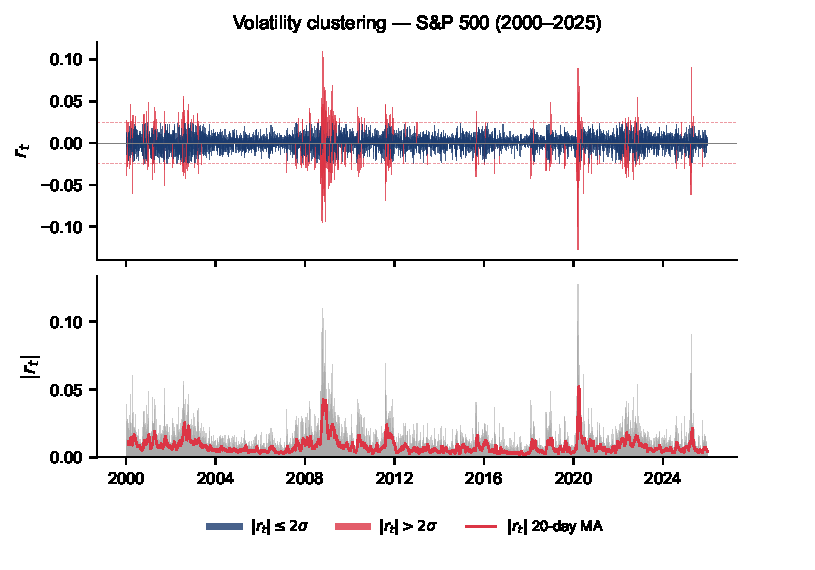
\includegraphics[width=\textwidth]{ch2_volatility_clustering.pdf}\\
\scriptsize\textit{Fig. 1: Randamente zilnice --- clustering vizibil în volatilitate.}
\end{center}
\end{column}
\end{columns}
\end{frame}

\begin{frame}[shrink=22]{P14. Rezolvare}
\begin{columns}[T]
\begin{column}{0.5\textwidth}
\begin{block}{(a) Stylized fact}
\textbf{Volatility clustering} (Mandelbrot 1963): „magnitudinile mari ale randamentelor tind să fie urmate de magnitudini mari, indiferent de semn''.

Matematic, $\Corr(r_t,r_{t-k})\approx 0$, dar:
\[
\Corr(|r_t|,|r_{t-k}|) > 0,\quad \Corr(r_t^2,r_{t-k}^2) > 0
\]
pe orizonturi $k$ de zeci de zile.
\end{block}
\begin{block}{(b) De ce nu i.i.d.\ Gaussian?}
\begin{itemize}\setlength{\itemsep}{0pt}
\item Sub i.i.d., $\sigma$ este constantă $\Rightarrow$ fără clustere de volatilitate.
\item În ipoteza distribuției Normale, kurtosis $=3$; empiric, kurtosis $\gg 3$.
\item VaR static (Normal cu $\sigma$ constant) ratează „spike-urile'' din perioadele de criză.
\end{itemize}
\end{block}
\end{column}
\begin{column}{0.48\textwidth}
\begin{block}{(c) Modele care captează clustering}
\textbf{Familia (G)ARCH} --- volatilitatea condiționată este dinamică:
\[
r_t = \mu + \varepsilon_t,\quad \varepsilon_t = \sigma_t\, z_t,\ z_t\overset{\text{i.i.d.}}{\sim}\mathcal D
\]
GARCH(1,1) (Bollerslev 1986):
\[
\sigma_t^2 = \omega + \alpha\,\varepsilon_{t-1}^2 + \beta\,\sigma_{t-1}^2
\]
\begin{itemize}\setlength{\itemsep}{0pt}
\item $\alpha+\beta<1$: staționaritate
\item $\alpha+\beta\to 1$: persistență mare (tipic 0.97--0.99)
\item Extensii: \textbf{GJR-GARCH}/EGARCH (efect de levier), \textbf{stochastic volatility}.
\end{itemize}
\end{block}
\begin{alertblock}{Verbatim de pus în răspuns}
„Volatility clustering'', „heteroscedasticitate condiționată'', „GARCH'', „kurtosis necondiționată generată endogen''.
\end{alertblock}
\end{column}
\end{columns}
\end{frame}

%---------- P15: Tail comparison ----------
\begin{frame}[shrink=15]{P15. Comparație cozi: empiric vs.\ Normal vs.\ Student vs.\ stable --- enunț}
\begin{columns}[T]
\begin{column}{0.45\textwidth}
\begin{block}{Enunț}
Pentru randamentele zilnice logaritmice ale indicelui S\&P500 s-au estimat trei modele parametrice ale distribuției --- Normal, Student-$t$ și $\alpha$-stable --- iar densitățile rezultate au fost reprezentate suprapus peste estimarea kernel (KDE) a distribuției empirice, pe scară log-y. Modelele au fost selectate prin minimizarea AIC; numărul de observații $n\approx 6500$.

\textbf{(a)} Pe baza graficului, care dintre cele trei modele parametrice descrie cel mai bine \emph{coada stângă} a distribuției? Justificați comparând comportamentul la $\log r \approx -0.10$.\\
\textbf{(b)} Ce model \emph{subestimează} cel mai grav riscul extrem? Calculați diferența dintre $\VaR^{99\%}$ în ipoteza distribuției Normale vs.\ Student-$t_4$ pentru $\sigma=2\%$.\\
\textbf{(c)} Indicați două criterii statistice pentru a alege formal modelul optim între aceste alternative și explicați limitele KS p-value pe eșantioane mari.
\end{block}
\end{column}
\begin{column}{0.53\textwidth}
\begin{center}
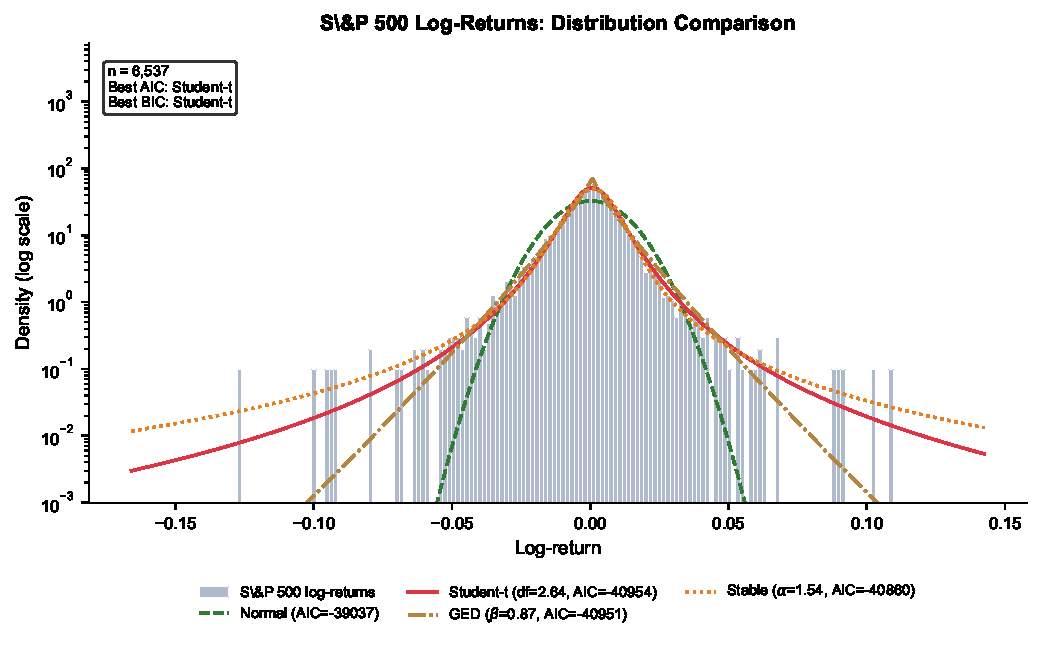
\includegraphics[width=\textwidth]{ch2_dist_comparison_overlay.pdf}\\
\scriptsize\textit{Fig. 2: Densitatea empirică vs.\ Normal, Student-$t$, $\alpha$-stable.}
\end{center}
\end{column}
\end{columns}
\end{frame}

\begin{frame}[shrink=22]{P15. Rezolvare}
\begin{columns}[T]
\begin{column}{0.5\textwidth}
\begin{block}{(a) Modelul cel mai adecvat}
Comparăm \emph{vizual} suprapunerea cu densitatea empirică (KDE):
\begin{itemize}\setlength{\itemsep}{0pt}
\item \textbf{Normal}: ratează atât \emph{peak}-ul central (prea jos), cât și cozile (prea ușoare).
\item \textbf{Student-$t$}: peak corect, cozi mai bune --- de obicei foarte aproape de empiric.
\item \textbf{$\alpha$-stable}: peak corect, cozi corecte, captează asimetria.
\end{itemize}
\textbf{Verdict}: $\alpha$-stable sau Student-$t$ cu DOF mic ($\sim 4$--6) sunt cele mai apropiate de empiric.
\end{block}
\begin{block}{(b) Model care subestimează}
\textbf{Normalul} subestimează cel mai grav coada stângă.

Pentru un randament cu $\sigma=2\%$:
\begin{itemize}\setlength{\itemsep}{0pt}
\item VaR\,99\% Normal: $-2.33\sigma=-4.66\%$
\item VaR\,99\% Student-$t_4$: $\sim -7\%$ (Student-$t$, $q_{0.01}\approx -3.75$)
\item Diferență $\sim 50\%$: capital de risc dramatic subestimat.
\end{itemize}
\end{block}
\end{column}
\begin{column}{0.48\textwidth}
\begin{block}{(c) Două criterii statistice}
\begin{enumerate}\setlength{\itemsep}{1pt}
\item \textbf{Criterii informaționale}: $\text{AIC} = -2\log L + 2k$, $\text{BIC} = -2\log L + k\log n$. Model cu \emph{cel mai mic} AIC/BIC este preferat. BIC penalizează mai dur complexitatea.
\item \textbf{Test goodness-of-fit}: Kolmogorov--Smirnov, Anderson--Darling, Cramér--von Mises. Sub $H_0$ (modelul este corect), statistica este mică; respingem dacă $p<0.05$.
\item Bonus: \textbf{QQ-plot} --- vizualizare cuantilă-cuantilă; modelul bun aliniază punctele pe diagonala $y=x$.
\item Bonus: testul \textbf{Likelihood Ratio} pentru modele nested (Normal $\subset$ Student-$t$).
\end{enumerate}
\end{block}
\begin{alertblock}{Capcană}
„KS p-value $<0.05$ pentru toate'' nu înseamnă că niciun model nu e bun: la $n$ mare ($>1000$) toate distribuțiile sunt respinse statistic. Folosiți AIC/BIC pentru \emph{ranking relativ}.
\end{alertblock}
\end{column}
\end{columns}
\end{frame}

%---------- P16: Hill plot ----------
\begin{frame}[shrink=20]{P16. Hill plot --- enunț}
\begin{columns}[T]
\begin{column}{0.45\textwidth}
\begin{block}{Enunț}
Pentru pierderile zilnice ($-r_t$ când $r_t<0$) ale indicelui S\&P500 s-a construit Hill plot al estimatorului indexului Pareto $\hat\alpha_k$, ca funcție de numărul $k$ al statisticilor de ordine cele mai mari incluse în estimare (în partea stângă, scară liniară; în dreapta, plot log-log al funcției de supraviețuire empirică cu fit Pareto suprapus). În zona de stabilitate se citește $\hat\alpha\approx 3.5$.

\textbf{(a)} Definiți formal estimatorul Hill și explicați cum se interpretează \emph{zona de plateau} pe Hill plot pentru alegerea unei valori robuste a lui $\hat\alpha$.\\
\textbf{(b)} Pentru $\hat\alpha\approx 3.5$, stabiliți care momente există (medie, varianță, skewness, kurtosis) și discutați consecințele practice pentru estimarea \emph{empirică} a varianței eșantion.\\
\textbf{(c)} Comparați probabilitatea unei pierderi $>5\sigma$ într-o singură zi sub modelul Pareto-tail cu $\hat\alpha=3.5$ și sub modelul Normal calibrat. Interpretați diferența în zile/ani de revenire.
\end{block}
\end{column}
\begin{column}{0.53\textwidth}
\begin{center}
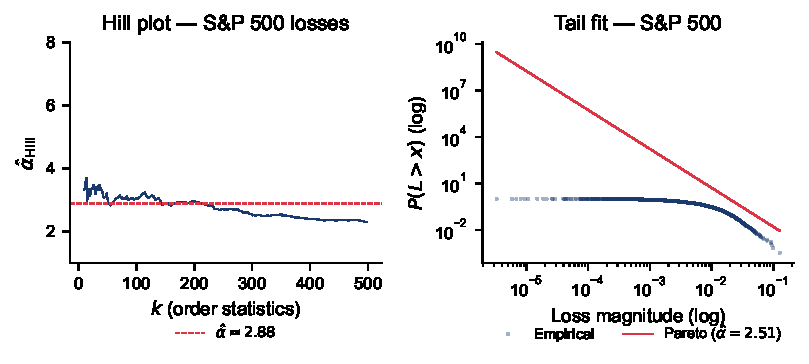
\includegraphics[width=\textwidth]{ch2_pareto_hill_sp500.pdf}\\
\scriptsize\textit{Fig. 3: Hill plot pe S\&P500 (coada stângă).}
\end{center}
\end{column}
\end{columns}
\end{frame}

\begin{frame}[shrink=35]{P16. Rezolvare}
\begin{columns}[T]
\begin{column}{0.5\textwidth}
\begin{block}{(a) Estimatorul Hill}
Fie $X_{(1)}\geq X_{(2)}\geq \dots\geq X_{(n)}$ statisticile de ordine descrescătoare. Estimatorul Hill (1975) pentru indexul Pareto $\alpha$, bazat pe primele $k$ extreme:
\[
\hat\alpha_k = \left[\frac{1}{k}\sum_{i=1}^{k}\ln X_{(i)} - \ln X_{(k+1)}\right]^{-1}
\]
\textbf{Citire pe grafic}: alegem o \emph{zonă de stabilitate} (plateau) pe Hill plot --- $\hat\alpha$ aproximativ constant pe un interval mediu de $k$. Pe S\&P500, plateau-ul tipic este la $\hat\alpha\in[3,4]$.
\end{block}
\begin{block}{(b) Existența momentelor}
Pentru Pareto de coadă $\alpha$, momentul de ordin $r$ există $\Leftrightarrow$ $r<\alpha$.

Cu $\hat\alpha\approx 3.5$:
\begin{itemize}\setlength{\itemsep}{0pt}
\item Media $r=1<3.5$ \correct
\item Varianța $r=2<3.5$ \correct
\item Skewness $r=3<3.5$ \correct (la limită)
\item Kurtosis $r=4>3.5$ \incorrect{} \textbf{infinit}
\end{itemize}
\textbf{Consecință}: varianța \emph{eșantion} converge la o limită finită (legea numerelor mari), dar foarte \emph{lent} --- estimările sunt instabile, fluctuează la apariția fiecărei valori extreme.
\end{block}
\end{column}
\begin{column}{0.48\textwidth}
\begin{block}{(c) Probabilitate pierdere $>5\sigma$}
\textbf{În ipoteza distribuției Normale}:
\[
P(Z<-5) = 1 - \Phi(5) \approx 2.87\cdot 10^{-7}
\]
$\Rightarrow$ 1 eveniment la $\sim 3.5\cdot 10^6$ zile $\approx$ \textbf{13{,}800 ani}.
\\[0.2em]
\textbf{Sub Pareto cu $\alpha=3.5$} (calibrat astfel încât evenimentul de $1\sigma$ să aibă aceeași prob.\ ca în Normal):
\[
P(|X|>5\sigma) = (1/5)^{3.5} = 0.2^{3.5} \approx 0.00358
\]
$\Rightarrow$ 1 eveniment la $\sim 280$ zile $\approx$ \textbf{aproape anual}.
\\[0.4em]
\textbf{Diferență}: factor $\sim 10^4$. De aici comentariul Goldman cu „25 abateri'' din P5: sub cozi grele, evenimentele extreme sunt cu ordine de mărime mai frecvente.
\end{block}
\end{column}
\end{columns}
\end{frame}

%---------- P17: Stable PDFs ----------
\begin{frame}[shrink=25]{P17. Densități $\alpha$-stable --- enunț}
\begin{columns}[T]
\begin{column}{0.42\textwidth}
\begin{block}{Enunț}
Graficul alăturat prezintă densitățile $\alpha$-stable simetrice (cu $\beta=0$, $\gamma=1$, $\delta=0$) pentru patru valori ale indexului de stabilitate $\alpha\in\{0.5, 1.0, 1.5, 2.0\}$, în scară liniară (stânga) și log-y (dreapta). Familia $\alpha$-stable apare natural ca limită în Teorema Limită Centrală Generalizată (Gnedenko--Kolmogorov) pentru sume de variabile aleatoare cu cozi grele.

\textbf{(a)} Asociați fiecărei curbe valoarea corespunzătoare a lui $\alpha$ și identificați \emph{numele clasic} al celor patru cazuri ($\alpha=2$, $\alpha=1.5$, $\alpha=1$, $\alpha=0.5$ cu $\beta=1$).\\
\textbf{(b)} Descrieți efectul scăderii lui $\alpha$ asupra a trei caracteristici ale densității: înălțimea peak-ului central, „umerii'' distribuției și grosimea cozilor (cu specificarea ratei de descreștere $P(|X|>x)$).\\
\textbf{(c)} Pentru randamente cripto (BTC, ETH) s-a estimat empiric $\alpha\in[1.5, 1.8]$. Justificați alegerea modelului $\alpha$-stable prin CLT generalizată și comparați cu Student-$t$ din punct de vedere al \emph{proprietății de stabilitate} sub sumare.
\end{block}
\end{column}
\begin{column}{0.56\textwidth}
\begin{center}
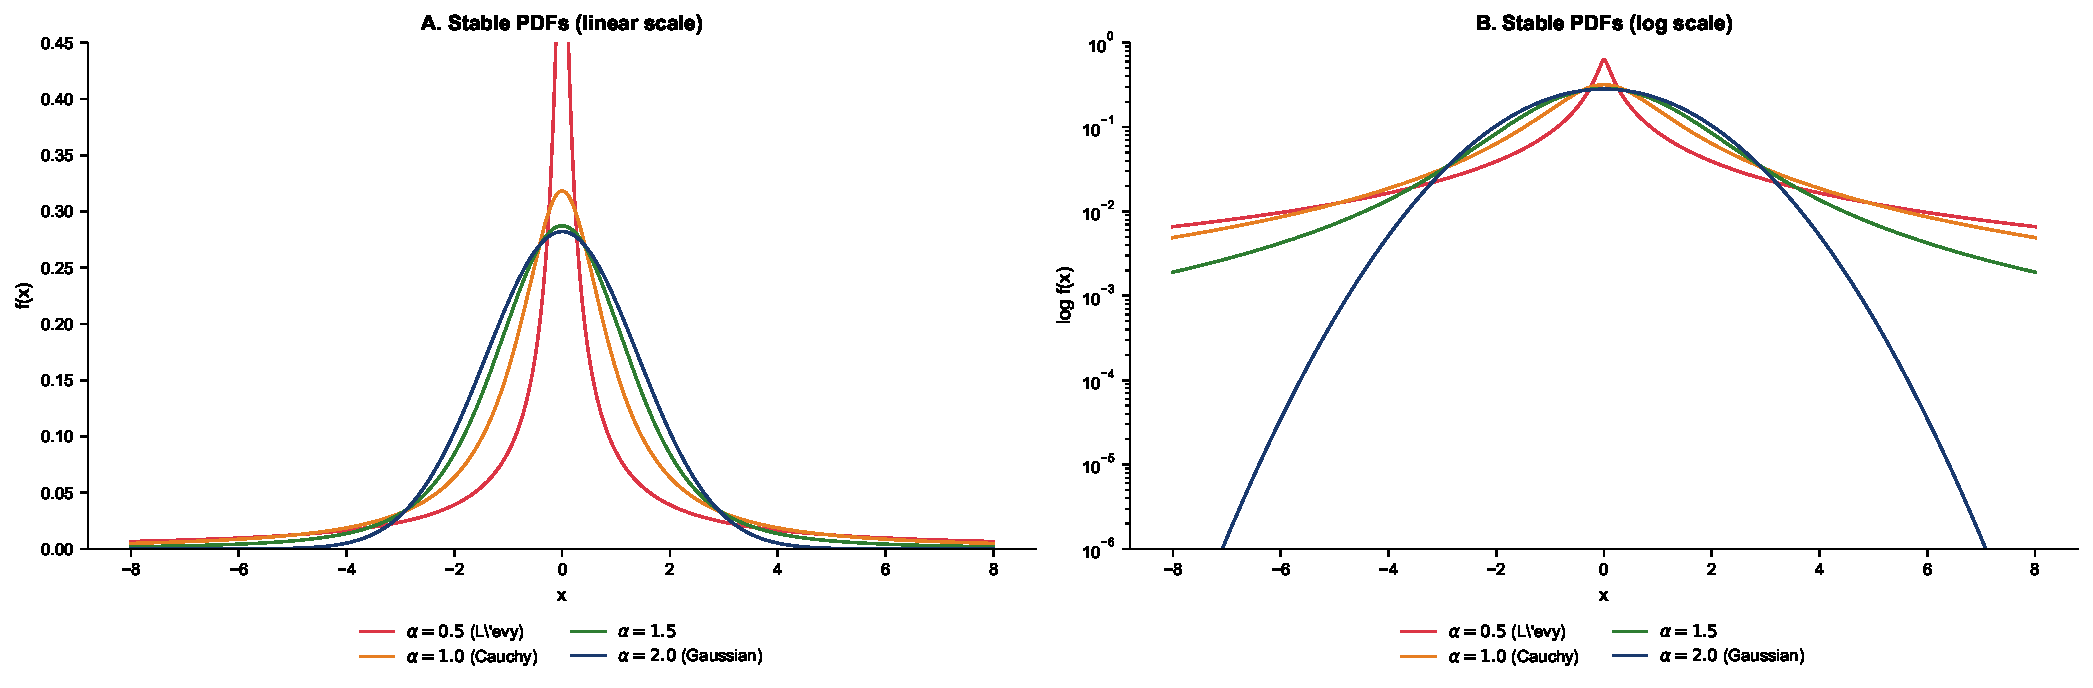
\includegraphics[width=\textwidth]{ch2_stable_pdfs.pdf}\\
\scriptsize\textit{Fig. 4: Densități $\alpha$-stable simetrice pentru diferite $\alpha$.}
\end{center}
\end{column}
\end{columns}
\end{frame}

\begin{frame}[shrink=22]{P17. Rezolvare}
\begin{columns}[T]
\begin{column}{0.5\textwidth}
\begin{block}{(a) Identificare curbe \& cazuri clasice}
\begin{itemize}\setlength{\itemsep}{1pt}
\item $\alpha=2.0$: \textbf{Normal} ($\sigma^2=2\gamma^2$) --- peak mediu, cozi gaussiene.
\item $\alpha=1.5$: \textbf{Holtsmark} (folosită în astrofizică pentru câmpurile gravitaționale stelare; valoare empirică tipică pentru cripto BTC/ETH).
\item $\alpha=1.0$: \textbf{Cauchy} (cu $\delta=0$, $\gamma=1$) --- peak mai înalt, cozi $\propto 1/x^2$.
\item $\alpha=0.5$: \textbf{Lévy} (one-sided dacă $\beta=1$) --- peak foarte înalt, cozi extrem de grele.
\end{itemize}
\end{block}
\begin{block}{(b) Efectul scăderii lui $\alpha$}
\begin{itemize}\setlength{\itemsep}{0pt}
\item \textbf{Peak central}: \emph{crește în înălțime} (concentrare mai mare în jurul medianei).
\item \textbf{Cozile}: \emph{se îngroașă} --- $P(|X|>x)\sim x^{-\alpha}$ pentru $\alpha<2$.
\item \textbf{Umerii} („shoulders''): se subțiază --- distribuția devine „pointy-tailed''.
\item \textbf{Varianța}: $\infty$ pentru $\alpha<2$; media $\infty$ pentru $\alpha\leq 1$.
\end{itemize}
\end{block}
\end{column}
\begin{column}{0.48\textwidth}
\begin{block}{(c) Cripto $\Rightarrow$ $\alpha\in[1.5,1.8]$}
\textbf{CLT generalizată (Gnedenko--Kolmogorov)}: suma normalizată de v.a.\ i.i.d.\ cu cozi de tipul Pareto cu index $\alpha<2$ converge la o \emph{lege $\alpha$-stable}, NU la o Normală.

\textbf{Aplicație BTC/ETH}:
\begin{itemize}\setlength{\itemsep}{0pt}
\item Randamente zilnice cripto au cozi de tip $\alpha\approx 1.6$--$1.8$ (estimat empiric).
\item Sumarea zilnică (e.g., randament săptămânal) păstrează indexul $\alpha$ (proprietatea de stabilitate).
\item Modelul $\alpha$-stable este \emph{teoretic justificat}, nu doar empiric.
\end{itemize}
\textbf{Comparație cu Student-$t$}: Student-$t_\nu$ are cozi grele dar NU este stabilă sub sumare. Suma de Student-$t$ tinde tot la Normal sub CLT clasică.
\end{block}
\end{column}
\end{columns}
\end{frame}

%---------- P18: Markowitz efficient frontier ----------
\begin{frame}[shrink=22]{P18. Frontiera eficientă Markowitz --- enunț}
\begin{columns}[T]
\begin{column}{0.42\textwidth}
\begin{block}{Enunț}
Graficul alăturat prezintă rezultatele optimizării medie-varianță pentru un univers de 3 active riscante (AAPL, GLD, BTC). Norul de puncte colorat reprezintă portofolii aleatoare cu ponderi $w\geq 0$, $\sum w_i=1$; culoarea codifică indicatorul Sharpe. Curba neagră este frontiera eficientă (efficient frontier), iar punctul roșu este portofoliul tangent calculat cu rată fără risc $r_f=0$. Steluța neagră marchează MVP (minimum variance portfolio).

\textbf{(a)} Definiți formal frontiera eficientă ca soluție a unei probleme de optimizare. Argumentați de ce \emph{ramura inferioară} (sub MVP) este sub-optimă în sens stochastic.\\
\textbf{(b)} Citiți din grafic coordonatele aproximative $(\sigma, \mu)$ pentru: (i) portofoliul MVP; (ii) portofoliul tangent.\\
\textbf{(c)} Calculați indicatorul Sharpe pentru portofoliul tangent. Discutați semnificația prin teorema separației lui Tobin și conceptul de Capital Market Line (CML).
\end{block}
\end{column}
\begin{column}{0.56\textwidth}
\begin{center}
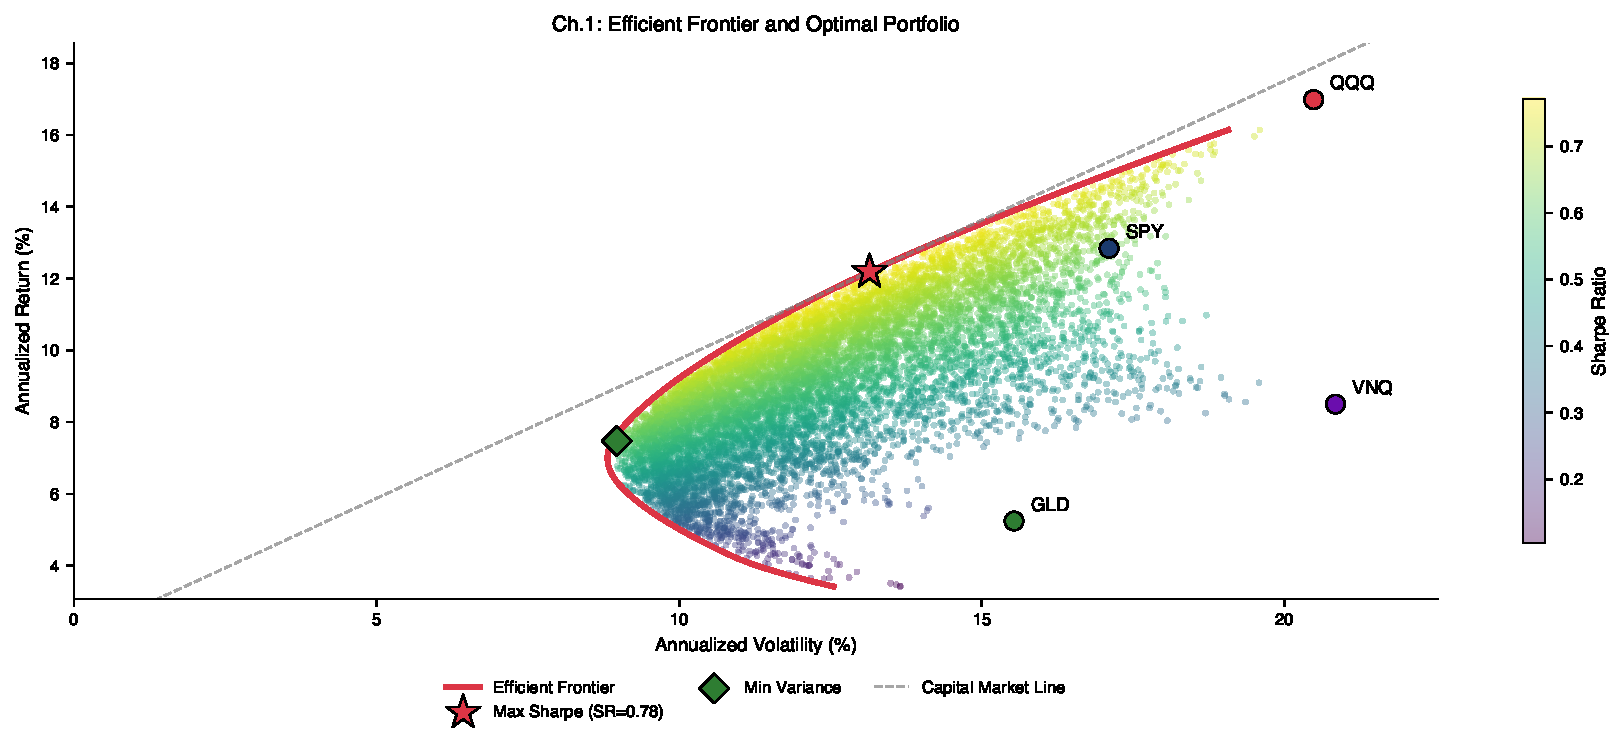
\includegraphics[width=\textwidth]{ch1_efficient_frontier.pdf}\\
\scriptsize\textit{Fig. 5: Frontiera eficientă \& portofoliu tangent.}
\end{center}
\end{column}
\end{columns}
\end{frame}

\begin{frame}[shrink=22]{P18. Rezolvare}
\begin{columns}[T]
\begin{column}{0.5\textwidth}
\begin{block}{(a) Frontiera eficientă}
\textbf{Definiție}: locul portofoliilor cu \emph{varianță minimă} pentru un nivel dat al rentabilității medii. Formal:
\[
\min_w \frac{1}{2} w^\top \Sigma w \quad\text{s.t.}\ w^\top \mu = \bar r,\ w^\top \mathbf{1}=1
\]
\textbf{Porțiunea inferioară este sub-optimă}: pentru același risc $\sigma$, există un portofoliu pe ramura superioară cu rentabilitate \emph{strict mai mare} $\Rightarrow$ \emph{dominată stochastic de ordin 1}. Investitorii raționali aleg numai ramura superioară.
\end{block}
\begin{block}{(b) Coordonate MVP \& tangent (citire grafic)}
\begin{itemize}\setlength{\itemsep}{0pt}
    \item \textbf{MVP}: punctul de cea mai mică abscisă pe frontieră, e.g., $(\sigma, \mu)\approx(0.12, 0.04)$.
    \item \textbf{Tangent} (punctul roșu): unde tangenta din $(0, r_f=0)$ atinge frontiera, e.g., $(\sigma_T, \mu_T)\approx(0.18, 0.10)$.
\end{itemize}
\end{block}
\end{column}
\begin{column}{0.48\textwidth}
\begin{block}{(c) Indicatorul Sharpe --- portofoliul tangent}
\[
\text{Sharpe}_T = \frac{\mu_T - r_f}{\sigma_T} = \frac{0.10 - 0}{0.18} \approx \mathbf{0.56}
\]
\textbf{Semnificație}:
\begin{itemize}\setlength{\itemsep}{0pt}
\item Indicatorul Sharpe = randament excedentar per unitate de risc.
\item Portofoliul tangent are \emph{cea mai mare valoare a indicatorului Sharpe} pe frontieră (teorema separației Tobin).
\item Combinând tangentul cu activul fără risc obținem \emph{Capital Market Line} (CML), care domină frontiera originală.
\item Sharpe $>0.5$ anualizat este considerat „bun''; $>1$ este excelent (rar în practică net de costuri).
\end{itemize}
\end{block}
\begin{alertblock}{Capcană}
Indicatorul Sharpe presupune randamente \emph{normal-distribuite}. Pentru cripto/active leptokurtice, folosiți \textbf{Sortino} (penalizează doar downside) sau \textbf{Calmar} (raport la max drawdown).
\end{alertblock}
\end{column}
\end{columns}
\end{frame}

%---------- P19: Random walk prediction ----------
\begin{frame}{P19. Predicție prețuri sub random walk --- enunț}
\begin{block}{Enunț}
Un analist financiar modelează prețul zilnic de închidere al unei acțiuni listate la BVB printr-un proces de tip \emph{random walk cu drift zero și volatilitate constantă}:
\[
P_t = P_{t-1} + 2\,\varepsilon_t,\quad \varepsilon_t \overset{\text{i.i.d.}}{\sim} \mathcal N(0,1)
\]
unde $\varepsilon_t$ reprezintă \emph{inovația} (noua informație care ajunge pe piață în ziua $t$). La închiderea zilei curente $t$, prețul observat este $P_t = 12.5$ lei.

\textbf{(a)} Determinați \emph{cea mai bună predicție} (în sens MSE minim) a prețului la momentul $t+1$ și explicați raționamentul.\\
\textbf{(b)} Construiți intervalul de încredere 95\% pentru $P_{t+1}$. Discutați cum se schimbă lățimea IC pe un orizont $T$ zile (relația $\sqrt T$).\\
\textbf{(c)} Interpretați rezultatele în contextul ipotezei de piață eficientă (forma slabă). Ce strategii de tranzacționare sunt compatibile cu acest model?
\end{block}
\end{frame}

\begin{frame}[shrink=22]{P19. Rezolvare}
\begin{columns}[T]
\begin{column}{0.5\textwidth}
\begin{block}{(a) Cea mai bună predicție}
Cea mai bună predicție în sensul \emph{MSE minim} (predictor punctual optim) este \emph{media condiționată}:
\[
\hat P_{t+1\mid t} = \E[P_{t+1}\mid \mathcal F_t] = P_t + 2\,\E[\varepsilon_{t+1}\mid \mathcal F_t]
\]
Deoarece $\varepsilon_{t+1}$ este viitor și independent de $\mathcal F_t$, $\E[\varepsilon_{t+1}]=0$:
\[
\boxed{\hat P_{t+1\mid t} = P_t = \mathbf{12.5\ \text{lei}}}
\]
\textbf{Concluzie}: cea mai bună predicție pentru ziua de mâine este \emph{prețul de azi} --- proprietatea de \emph{martingală}.
\end{block}
\begin{block}{(b) Interval de încredere 95\%}
$P_{t+1}\mid\mathcal F_t \sim \mathcal N(P_t, 4)$ (varianța $= 4\cdot 1=4$).
\[
\text{IC}_{95\%} = P_t \pm 1.96\cdot \sigma = 12.5 \pm 1.96\cdot 2
\]
\[
\boxed{\text{IC}_{95\%} = [\mathbf{8.58,\ 16.42}]\ \text{lei}}
\]
\end{block}
\end{column}
\begin{column}{0.48\textwidth}
\begin{block}{(c) Interpretare EMH}
Modelul $P_t = P_{t-1} + 2\varepsilon_t$ este un \textbf{random walk cu varianță 4}. Implicații:
\begin{itemize}\setlength{\itemsep}{0pt}
\item \emph{Inovațiile} $\varepsilon_t$ sunt informația nouă care ajunge pe piață --- imprevizibile.
\item Cea mai bună predicție = prețul curent $\Rightarrow$ \textbf{nicio strategie tehnică} (medii mobile, momentum, etc.) nu poate face mai bine decât „buy-and-hold''.
\item Modelul este consistent cu \textbf{EMH forma slabă}: prețurile încorporează toată informația din istoricul prețurilor.
\item Intervalul de încredere se lățește cu $\sqrt T$: $\text{IC}_{T} = P_t \pm 1.96\cdot 2\sqrt T$ --- incertitudinea crește cu orizontul.
\end{itemize}
\end{block}
\begin{alertblock}{Capcană}
„Cea mai bună predicție = ultimul preț observat'' \emph{NU} înseamnă că prețul nu se va schimba --- înseamnă că \emph{modificarea sa medie este zero}. Volatilitatea este pozitivă ($\sigma=2$).
\end{alertblock}
\end{column}
\end{columns}
\end{frame}

%---------- P20: Variance Ratio plot reading ----------
\begin{frame}[shrink=22]{P20. Variance Ratio plot --- enunț}
\begin{columns}[T]
\begin{column}{0.42\textwidth}
\begin{block}{Enunț}
Pentru testarea ipotezei de eficiență slabă (random walk) a unui activ financiar s-a aplicat \emph{Variance Ratio Test} (Lo \& MacKinlay 1988) pe diferite orizonturi de agregare $q$. În stânga (Panel A) este reprezentată statistica $VR(q)$ ca funcție de $q$, cu intervalul de încredere 95\% (linia roșie punctată); în dreapta (Panel B), $VR(q)$ pe ferestre mobile de 200 zile pentru a vedea evoluția în timp a (in)eficienței.

\textbf{(a)} Formulați ipoteza nulă $H_0$ a testului VR și indicați regula de decizie. Pe baza Panel A, pentru ce orizonturi $q$ \emph{respingem} $H_0$ la pragul de 5\%?\\
\textbf{(b)} Interpretați economic direcția deviației: $VR(q)<1$ vs.\ $VR(q)>1$. Care este implicația asupra autocorelației de ordin scurt?\\
\textbf{(c)} Ce strategie de tranzacționare (contrarian sau trend-following) este sugerată de rezultate? Discutați cel puțin trei limitări practice (costuri, stabilitate temporală, multiple testing).
\end{block}
\end{column}
\begin{column}{0.56\textwidth}
\begin{center}
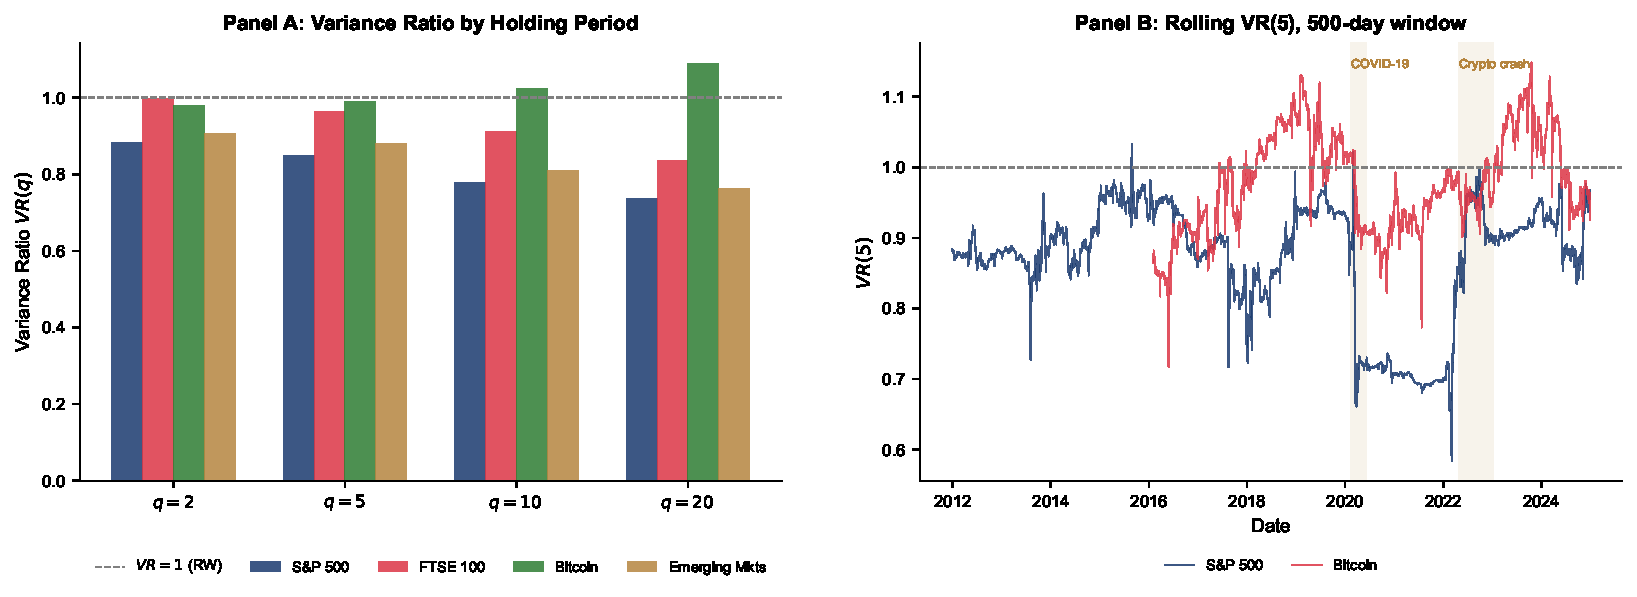
\includegraphics[width=\textwidth]{ch3_variance_ratio.pdf}\\
\scriptsize\textit{Fig. 7: Variance Ratio $VR(q)$ cu IC 95\%.}
\end{center}
\end{column}
\end{columns}
\end{frame}

\begin{frame}[shrink=22]{P20. Rezolvare}
\begin{columns}[T]
\begin{column}{0.5\textwidth}
\begin{block}{(a) Respingere $H_0$}
\textbf{Regulă de citire}: respingem $H_0: VR(q)=1$ la $\alpha=5\%$ dacă valoarea $VR(q)$ \emph{iese din banda de încredere} (linia roșie punctată):
\begin{itemize}\setlength{\itemsep}{0pt}
\item Dacă curba $VR(q)$ rămâne între LCL și UCL pentru toate $q$ $\Rightarrow$ \textbf{nu respingem} $H_0$ la niciun orizont $\Rightarrow$ activ consistent cu martingală.
\item Dacă iese în jos ($VR<\text{LCL}$): autocorelație negativă \emph{semnificativă}.
\item Dacă iese în sus ($VR>\text{UCL}$): autocorelație pozitivă \emph{semnificativă}.
\end{itemize}
\end{block}
\begin{block}{(b) Direcția deviației}
\begin{itemize}\setlength{\itemsep}{0pt}
\item $VR(q)<1$: \textbf{mean-reversion} --- după o creștere urmează probabil o scădere (corelație serială negativă). Tipic acțiuni mature, indici largi.
\item $VR(q)>1$: \textbf{momentum} --- trend-following profitabil pe termen scurt. Tipic emerging markets, cripto la început de cariera, small-caps.
\item $VR(q)=1$: random walk, nicio predictibilitate liniară.
\end{itemize}
\end{block}
\end{column}
\begin{column}{0.48\textwidth}
\begin{block}{(c) Strategie sugerată \& limitări}
\textbf{Dacă $VR<1$ (mean reversion)}:
\begin{itemize}\setlength{\itemsep}{0pt}
\item Strategie \emph{contrarian}: vinde după creștere mare, cumpără după scădere mare.
\item Pair trading, statistical arbitrage.
\end{itemize}
\textbf{Dacă $VR>1$ (momentum)}:
\begin{itemize}\setlength{\itemsep}{0pt}
\item Strategie \emph{trend-following}: cross-uri de medii mobile, breakout-uri.
\end{itemize}
\textbf{Limitări critice}:
\begin{itemize}\setlength{\itemsep}{0pt}
\item Costuri de tranzacționare (spread, comisioane) pot anula întreaga semnal.
\item Stabilitatea este \emph{in-sample}; out-of-sample, $VR$ se schimbă în timp.
\item Volatilitate-clustering: chiar și sub $VR=1$, riscul condiționat nu este constant.
\item Selection bias: dacă testezi 100 active, $\sim 5$ vor părea semnificative pur prin întâmplare.
\end{itemize}
\end{block}
\end{column}
\end{columns}
\end{frame}

%---------- P21: GARCH conditional volatility ----------
\begin{frame}[shrink=25]{P21. GARCH(1,1) --- volatilitate condiționată din grafic}
\begin{columns}[T]
\begin{column}{0.42\textwidth}
\begin{block}{Enunț}
În graficul alăturat sunt reprezentate randamentele zilnice ale unui indice bursier (linie gri) pe o fereastră de aproximativ 1500 zile de tranzacționare, suprapuse cu $-\VaR^{99\%}$ estimat dinamic prin două abordări: (i) GARCH(1,1) cu inovații Normale (linie roșie) și (ii) Historical Simulation pe fereastră mobilă de $h=500$ zile (linie albastră). Punctele care depășesc banda $-\VaR$ reprezintă \emph{failures} (excepții).

\textbf{(a)} Explicați de ce $\VaR_t^{\text{GARCH}}$ este \emph{dinamic} și variază substanțial în timp, în timp ce un $\VaR^{\text{Normal-static}}$ calculat pe întreaga fereastră ar fi constant. Scrieți relația de bază.\\
\textbf{(b)} Identificați pe grafic perioadele de \emph{stress} (criza COVID, mini-crize 2018) și descrieți comportamentul $\sigma_t$. Care model reacționează mai rapid: GARCH sau Historical Simulation?\\
\textbf{(c)} Comparați \emph{reactivitatea} celor două modele la șocurile observate (criza COVID, mini-crize 2018): care reacționează \emph{instant} și care reacționează \emph{întârziat}? Care este consecința practică pentru un risk manager care reportează VaR zilnic la Comitetul de Risc?
\end{block}
\end{column}
\begin{column}{0.56\textwidth}
\begin{center}
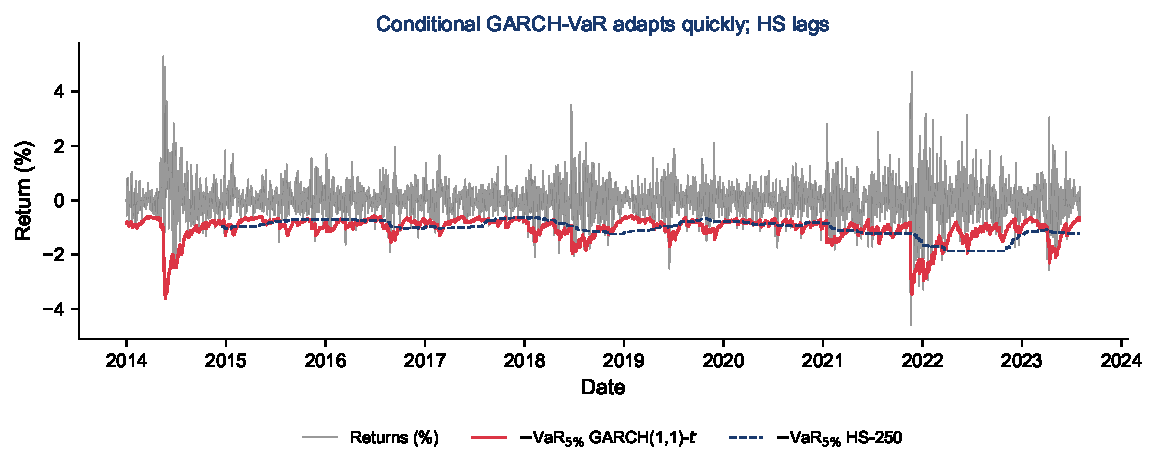
\includegraphics[width=\textwidth]{ch11_garch_var.pdf}\\
\scriptsize\textit{Fig. 8: Randamente și VaR\,99\% rolling GARCH(1,1).}
\end{center}
\end{column}
\end{columns}
\end{frame}

\begin{frame}[shrink=30]{P21. Rezolvare}
\begin{columns}[T]
\begin{column}{0.5\textwidth}
\begin{block}{(a) De ce $\VaR^{\text{GARCH}}$ este dinamic}
\textbf{VaR Normal static}: $\sigma$ estimată o singură dată pe întreaga fereastră $\Rightarrow$ constantă.
\[
\VaR^{\text{Normal,static}} = -2.33\cdot \hat\sigma = \text{const}
\]
\textbf{VaR GARCH}: $\sigma_t$ recalculată \emph{în fiecare zi} pe baza dinamicii:
\[
\sigma_t^2 = \omega + \alpha\,\varepsilon_{t-1}^2 + \beta\,\sigma_{t-1}^2
\]
\[
\VaR_t^{\text{GARCH}} = -2.33\cdot \sigma_t
\]
Astfel, $\VaR_t$ \emph{urmărește} regimurile de volatilitate: crește în crize, scade în perioade calme.
\end{block}
\begin{block}{(b) Perioade de stress}
Vizual, identificăm \emph{spike-uri} în VaR GARCH corespunzătoare crizelor:
\begin{itemize}\setlength{\itemsep}{0pt}
\item COVID (Mar 2020): $\sigma_t$ crește brusc, VaR ajunge la $-15\%$ sau mai jos.
\item Mini-crize (Aug 2015, Feb 2018, Dec 2018): vârfuri mai mici.
\item Perioade calme (2017, mid-2019): VaR \emph{ridicat} (less negative), $\sim -1.5\%$.
\end{itemize}
\end{block}
\end{column}
\begin{column}{0.48\textwidth}
\begin{block}{(c) Reactivitate GARCH vs.\ HS}
\textbf{GARCH(1,1)} --- reacție \emph{instantă}:
\begin{itemize}\setlength{\itemsep}{0pt}
\item După un șoc $\varepsilon_t^2$ mare, $\sigma_{t+1}^2$ crește imediat ($\alpha\,\varepsilon_t^2$).
\item Pe grafic: VaR-GARCH coboară abrupt la începutul COVID.
\end{itemize}
\textbf{Historical Simulation ($h=500$)} --- reacție \emph{întârziată}:
\begin{itemize}\setlength{\itemsep}{0pt}
\item Folosește cuantila empirică pe fereastra glisantă $\Rightarrow$ trebuie să se acumuleze suficiente observații extreme.
\item Pe grafic: VaR-HS coboară lin, cu întârziere $\sim 50$--$100$ zile.
\end{itemize}
\textbf{Consecință risk management}: GARCH avertizează \emph{înainte} de a se materializa pierderile mari $\Rightarrow$ permite reducerea expunerii \emph{preventiv}. HS reflectă riscul \emph{după} ce el a apărut --- bun pentru raportare ex-post, slab pentru decizii ex-ante.
\end{block}
\begin{alertblock}{Avantaj GARCH vs.\ static}
GARCH \emph{anticipează} creșterea riscului: după primul șoc mare, $\sigma_{t+1}$ explodează deja $\Rightarrow$ VaR mai prudent. Static-Normal continuă să dea aceeași valoare conservatoare/optimistă greșit.
\end{alertblock}
\end{column}
\end{columns}
\end{frame}

%---------- P22: Theory question — EMH vs FMH ----------
\begin{frame}{P22. Subiect de teorie: EMH vs.\ FMH --- enunț}
\begin{block}{Enunț}
Două paradigme concurente descriu comportamentul piețelor financiare: \emph{ipoteza pieței eficiente} (EMH, Fama 1970) și \emph{ipoteza pieței fractale} (FMH, Peters 1994). Pe baza cursului și a literaturii financiare clasice:

\textbf{(a)} Enunțați formele \emph{slabă}, \emph{semi-tare} și \emph{tare} ale EMH (Fama). Pentru fiecare, indicați tipul de informație care \emph{nu poate} aduce profituri sistematice excedentare.\\
\textbf{(b)} Enunțați cei trei piloni ai FMH (Peters): rolul investitorilor cu \emph{orizonturi diferite}, conceptul de \emph{memorie de lungă durată} ($H>0.5$), și relația dintre \emph{lichiditate} și \emph{stabilitate}.\\
\textbf{(c)} Argumentați două \emph{avantaje} și două \emph{dezavantaje} ale FMH în raport cu EMH, din perspectiva risk management-ului post-2008.
\end{block}
\end{frame}

\begin{frame}[shrink=25]{P22. Rezolvare}
\begin{columns}[T]
\begin{column}{0.5\textwidth}
\begin{block}{(a) Cele trei forme ale EMH}
\begin{itemize}\setlength{\itemsep}{1pt}
    \item \textbf{Slabă}: prețurile reflectă toată \emph{istoria prețurilor și volumelor}. Implică: \emph{analiza tehnică} nu poate produce profituri excedentare.
    \item \textbf{Semi-tare}: prețurile reflectă toată \emph{informația publică} (rapoarte anuale, știri, indicatori macro). Implică: \emph{analiza fundamentală} pe informație publică nu funcționează.
    \item \textbf{Tare}: prețurile reflectă \emph{toată} informația, inclusiv \emph{insider info}. Implică: nici insider trading nu produce profit (în formă pură, contrazis empiric).
\end{itemize}
\textbf{Test empiric}: VR test, Ljung--Box, runs test (forma slabă); event studies (semi-tare); studii pe insiders (tare).
\end{block}
\begin{block}{(b) Cei trei piloni FMH (Peters)}
\begin{enumerate}\setlength{\itemsep}{1pt}
    \item \textbf{Heterogenitate orizonturi}: investitori cu orizonturi diferite (zi/an/decadă); stabilitatea = coexistența lor.
    \item \textbf{Memorie de lungă durată}: $H>0.5$ $\Rightarrow$ tendințe persistente, nu pur random walk.
    \item \textbf{Lichiditate $\to$ stabilitate}: criza = retragerea orizonturilor lungi $\Rightarrow$ colaps de diversitate temporală.
\end{enumerate}
\end{block}
\end{column}
\begin{column}{0.48\textwidth}
\begin{block}{(c) Avantaje FMH vs.\ EMH}
\textbf{Avantaje FMH}:
\begin{itemize}\setlength{\itemsep}{0pt}
    \item Explică \emph{cozile grele} și volatility clustering --- empirice, ignorate de EMH (care presupune Gaussian).
    \item Explică \emph{crizele endogene} (1987, 2008, COVID): pierdere de heterogenitate $\Rightarrow$ colapsul lichidității.
\end{itemize}
\textbf{Dezavantaje FMH}:
\begin{itemize}\setlength{\itemsep}{0pt}
    \item Mai puțin \emph{tractabilă matematic} (fără modele de optimizare clasice tip Markowitz).
    \item Implicații pentru \emph{policy} mai puțin clare (cum reglementezi orizonturi?).
\end{itemize}
\end{block}
\begin{alertblock}{Concluzie pentru risk management post-2008}
EMH + Gaussian \emph{subestimează} sistematic riscul de criză (VaR-Normal eșuează în COVID). FMH + cozi grele \emph{prezic} fragilitatea structurală a piețelor. \textbf{Basel III/IV} și \textbf{stress-testing} integrează deja elemente FMH (scenarii non-gaussiene, EVT, $\alpha$-stable).
\end{alertblock}
\end{column}
\end{columns}
\end{frame}

%---------- P23: Expected Shortfall (ES) ----------
\begin{frame}{P23. Expected Shortfall vs.\ Value at Risk --- enunț}
\begin{block}{Enunț}
Pentru un portofoliu de acțiuni s-au estimat parametrii distribuției randamentelor logaritmice zilnice: $\mu = 0$, $\sigma = 0.02$. Riscul portofoliului este monitorizat zilnic prin două măsuri: Value at Risk ($\VaR$) și Expected Shortfall ($\ES$), ambele la nivelul de încredere de 99\%.

\textbf{(a)} Definiți formal Expected Shortfall ($\ES_\alpha$) și explicați legătura sa cu $\VaR_\alpha$. De ce $\ES$ este preferat ca măsură de risc în reglementarea Basel III/IV?\\
\textbf{(b)} Calculați $\VaR^{99\%}$ și $\ES^{99\%}$ în ipoteza distribuției Normale. Folosiți $z_{0.01} = -2.33$ și $\phi(z_{0.01}) = 0.0267$ (densitatea Normală standard în $-2.33$).\\
\textbf{(c)} Discutați \emph{subaditivitatea}: dați un exemplu intuitiv în care $\VaR$ \emph{nu} este subaditiv, dar $\ES$ este. Ce înseamnă acest lucru pentru diversificarea portofoliului?
\end{block}
\end{frame}

\begin{frame}[shrink=40]{P23. Rezolvare}
\begin{columns}[T]
\begin{column}{0.5\textwidth}
\begin{block}{(a) Definiția ES și legătura cu VaR}
\textbf{Expected Shortfall} (Conditional VaR, Tail VaR):
\[
\ES_\alpha = \E[L \mid L > \VaR_\alpha]
\]
unde $L=-r$ este pierderea. Reprezintă \emph{pierderea medie condiționată} \emph{în coadă}, dincolo de $\VaR$.

\textbf{De ce ES > VaR în Basel III/IV}:
\begin{itemize}\setlength{\itemsep}{0pt}
    \item \textbf{Coerență} (Artzner et al.\ 1999): ES satisface toate cele 4 axiome ale unei măsuri coerente; VaR nu satisface \emph{subaditivitatea}.
    \item \textbf{Captează coada}: VaR ignoră complet pierderile dincolo de prag; ES le \emph{integrează}.
    \item Basel III FRTB (Fundamental Review of the Trading Book, 2019) înlocuiește VaR cu ES\,97.5\%.
\end{itemize}
\end{block}
\begin{block}{(b) Calcul în ipoteza distribuției Normale}
$\VaR^{99\%} = -(\mu + z_{0.01}\sigma) = -(0 + (-2.33)\cdot 0.02) = \mathbf{0.0466 = 4.66\%}$.

Formula ES în ipoteza distribuției Normale:
\[
\ES_\alpha = \mu + \sigma\cdot\frac{\phi(z_\alpha)}{\alpha}
\]
\[
\ES^{99\%} = 0 + 0.02\cdot\frac{0.0267}{0.01} = 0.02\cdot 2.67 = \mathbf{0.0534 = 5.34\%}
\]
Raport: $\ES/\VaR = 5.34/4.66 \approx 1.15$ în ipoteza distribuției Normale.
\end{block}
\end{column}
\begin{column}{0.48\textwidth}
\begin{block}{(c) Subaditivitate}
\textbf{Exemplu non-Subaditivitate VaR}: două portofolii cu pierderi disjuncte rare.
\begin{itemize}\setlength{\itemsep}{0pt}
    \item Portofoliu $X$: pierde $\$100$ cu prob.\ 0.8\%, altfel $0$.
    \item Portofoliu $Y$: pierde $\$100$ cu prob.\ 0.8\%, altfel $0$.
    \item Independente $\Rightarrow$ $X+Y$ pierde $\$100$ cu prob.\ $\approx 1.6\%$, $\$200$ cu prob.\ $\approx 0.006\%$.
\end{itemize}
La $\alpha=1\%$:
\[
\VaR_{X}=0,\ \VaR_{Y}=0,\ \VaR_{X+Y}=100
\]
$\Rightarrow \VaR_{X+Y} > \VaR_X + \VaR_Y$ --- \emph{diversificarea pare să mărească riscul}!
\end{block}
\begin{alertblock}{Concluzie}
ES respectă întotdeauna $\ES_{X+Y}\leq\ES_X + \ES_Y$ $\Rightarrow$ \emph{diversificarea nu poate niciodată mări ES}. Pentru cozi grele (Student-$t$, $\alpha$-stable), raportul $\ES/\VaR$ poate ajunge la 1.5--2.5. Folosirea VaR în Basel II a fost identificată drept slăbiciune în criza 2008.
\end{alertblock}
\end{column}
\end{columns}
\end{frame}

%---------- P24: Jarque-Bera test ----------
\begin{frame}{P24. Test Jarque--Bera de normalitate --- enunț}
\begin{block}{Enunț}
Pentru randamentele zilnice ale acțiunii TSLA pe o perioadă de $n=1{,}000$ zile de tranzacționare s-au calculat momentele eșantion: media $\bar r = 0$, abaterea standard $s = 0.04$, asimetria $\hat S = -0.50$, kurtosis-ul $\hat K = 5.20$. Pentru a verifica dacă randamentele urmează o distribuție Normală:

\textbf{(a)} Scrieți formula statisticii Jarque--Bera și ipoteza nulă $H_0$ testată. Specificați distribuția asimptotică sub $H_0$ și verificați compararea cu valoarea critică $\chi^2_{2;\,0.95} = 5.99$ la pragul de 5\%.\\
\textbf{(b)} Calculați valoarea statisticii JB pe baza momentelor de mai sus și decideți acceptarea/respingerea $H_0$.\\
\textbf{(c)} Comparați avantajele și dezavantajele JB față de Kolmogorov--Smirnov (KS) pentru testarea normalității randamentelor financiare.
\end{block}
\end{frame}

\begin{frame}[shrink=45]{P24. Rezolvare}
\begin{columns}[T]
\begin{column}{0.5\textwidth}
\begin{block}{(a) Formulă \& ipoteze}
\textbf{Statistica Jarque--Bera}:
\[
\text{JB} = \frac{n}{6}\left(\hat S^2 + \frac{(\hat K - 3)^2}{4}\right)
\]
\textbf{Ipoteze}:
\[
H_0:\ S=0\ \text{și}\ K=3\ (\text{normalitate})
\]
\[
H_1:\ S\neq 0\ \text{sau}\ K\neq 3
\]
\textbf{Distribuție asimptotică}: $\text{JB} \overset{d}{\to} \chi^2_2$ sub $H_0$.

\textbf{Valoarea critică} la 5\%: $\chi^2_{2;\,0.95} = \mathbf{5.99}$.

Regula: respingem $H_0$ dacă $\text{JB} > 5.99$.
\end{block}
\begin{block}{(b) Calcul numeric}
$\hat S^2 = (-0.50)^2 = 0.25$.

$(\hat K - 3)^2/4 = (5.20-3)^2/4 = 4.84/4 = 1.21$.

\[
\text{JB} = \frac{1000}{6}\cdot(0.25 + 1.21) = 166.67\cdot 1.46
\]
\[
\boxed{\text{JB} \approx \mathbf{243.3}}
\]
$243.3 \gg 5.99 \Rightarrow$ \textbf{respingem} $H_0$ cu certitudine ridicată (p-value $< 10^{-50}$).

\textbf{Concluzie}: randamentele TSLA \emph{nu} sunt Normale --- au cozi grele și asimetrie negativă.
\end{block}
\end{column}
\begin{column}{0.48\textwidth}
\begin{block}{(c) JB vs.\ KS}
\textbf{Avantaje JB}:
\begin{itemize}\setlength{\itemsep}{0pt}
    \item Captează direct \emph{cozile grele} (prin kurtosis) și \emph{asimetria}.
    \item Putere mare împotriva alternativelor leptokurtice (Student-$t$, stable).
    \item Foarte simplu de calculat dacă ai deja $\hat S$ și $\hat K$.
\end{itemize}
\textbf{Avantaje KS}:
\begin{itemize}\setlength{\itemsep}{0pt}
    \item Non-parametric, distribuție-independent.
    \item Testează \emph{întreaga distribuție}, nu doar 2 momente.
\end{itemize}
\textbf{Dezavantaje JB}: bazat pe asimptotică, putere slabă pentru $n$ mic; sensibil la outlieri extremi care distorsionează $\hat K$.

\textbf{Dezavantaje KS}: putere mai slabă la cozi; pe eșantioane mari ($n>1000$) respinge \emph{aproape orice} model parametric (chiar și unul „bun'').
\end{block}
\begin{alertblock}{Recomandare practică}
Folosiți AMÂNDOUĂ + QQ-plot pentru o concluzie robustă. JB pentru cozi/asimetrie, KS pentru forma globală.
\end{alertblock}
\end{column}
\end{columns}
\end{frame}

%---------- P25: Cornish-Fisher VaR ----------
\begin{frame}{P25. Cornish--Fisher VaR pentru distribuții non-normale --- enunț}
\begin{block}{Enunț}
Distribuția randamentelor unui portofoliu este aproape Normală dar cu \emph{asimetrie} și \emph{kurtosis în exces} ne-neglijabile. Pentru a obține un VaR mai realist fără a calibra o distribuție alternativă, s-a folosit expansiunea Cornish--Fisher (CF), care ajustează cuantila Normală folosind momentele superioare.

Pentru un portofoliu cu $\mu=0$, $\sigma = 0.02$, asimetrie $\hat S = -0.50$, kurtosis în exces $\hat K - 3 = 2.20$:

\textbf{(a)} Scrieți formula cuantilei Cornish--Fisher $z_{CF}$ în funcție de cuantila Normală $z_\alpha$, $\hat S$ și $\hat K - 3$.\\
\textbf{(b)} Calculați $\VaR^{99\%}$ folosind cuantila CF (pornind de la $z_{0.01} = -2.33$) și comparați cu $\VaR$ Normal standard.\\
\textbf{(c)} Discutați avantajele \& limitele aproximării CF față de calibrarea unei distribuții Student-$t$ sau $\alpha$-stable.
\end{block}
\end{frame}

\begin{frame}[shrink=40]{P25. Rezolvare}
\begin{columns}[T]
\begin{column}{0.5\textwidth}
\begin{block}{(a) Formula Cornish--Fisher}
Expansiunea Cornish--Fisher de ordin 4:
\begin{align*}
z_{CF} &= z_\alpha + \frac{z_\alpha^2 - 1}{6}\hat S + \frac{z_\alpha^3 - 3z_\alpha}{24}(\hat K - 3) \\
&\quad - \frac{2z_\alpha^3 - 5z_\alpha}{36}\hat S^2
\end{align*}
Termeni:
\begin{itemize}\setlength{\itemsep}{0pt}
    \item Termen 1: cuantila Normală
    \item Termen 2: corecție de \emph{asimetrie}
    \item Termen 3: corecție de \emph{kurtosis}
    \item Termen 4: corecție mixtă $\hat S^2$ (mai mică)
\end{itemize}
\end{block}
\begin{block}{(b) Calcul numeric ($\alpha=0.01$)}
$z_\alpha = -2.33$, $z_\alpha^2 = 5.43$, $z_\alpha^3 = -12.65$.

\textbf{Termen 2} (asimetrie): $\frac{5.43-1}{6}\cdot(-0.50) = \frac{4.43}{6}\cdot(-0.5) = -0.369$.

\textbf{Termen 3} (kurtosis): $\frac{-12.65-3\cdot(-2.33)}{24}\cdot 2.20 = \frac{-5.66}{24}\cdot 2.20 = -0.519$.

\textbf{Termen 4}: $-\frac{2\cdot(-12.65)-5\cdot(-2.33)}{36}\cdot 0.25 = -\frac{-13.65}{36}\cdot 0.25 = +0.0948$.

\[
z_{CF} = -2.33 - 0.369 - 0.519 + 0.0948 = -3.12
\]
\[
\VaR_{CF}^{99\%} = -(0 + (-3.12)\cdot 0.02) = \mathbf{0.0624 = 6.24\%}
\]
vs.\ $\VaR^{99\%}_{\text{Normal}} = 4.66\%$ --- \textbf{34\% mai mare}.
\end{block}
\end{column}
\begin{column}{0.48\textwidth}
\begin{block}{(c) CF vs.\ Student-$t$ / $\alpha$-stable}
\textbf{Avantaje CF}:
\begin{itemize}\setlength{\itemsep}{0pt}
    \item Calcul \emph{rapid și analitic}: necesită doar $\hat S$ și $\hat K$.
    \item Nu necesită calibrare iterativă (MLE).
    \item Standard în multe sisteme bancare comerciale.
    \item Bun pentru \emph{abateri mici} de la normalitate.
\end{itemize}
\textbf{Limite CF}:
\begin{itemize}\setlength{\itemsep}{0pt}
    \item Aproximare \emph{polinomială} --- proastă pentru cozi foarte grele.
    \item Poate da $z_{CF}$ \emph{non-monoton} în $\alpha$ pentru $|\hat S|$ sau $\hat K$ mari (paradox).
    \item Nu se aplică pentru $\hat K - 3 > 8$ (instabil).
\end{itemize}
\textbf{Recomandare}:
\begin{itemize}\setlength{\itemsep}{0pt}
    \item Student-$t$ / $\alpha$-stable pentru cozi grele (cripto, indici cu $\hat K > 10$).
    \item CF pentru abateri ușoare (acțiuni mature, $\hat K \in [3, 6]$).
\end{itemize}
\end{block}
\end{column}
\end{columns}
\end{frame}

%=============================================================================
% PARTEA VI: PROBLEME PROPUSE
%=============================================================================
\section{Partea VI --- Probleme propuse (fără soluții)}

\begin{frame}[shrink=22]{Probleme propuse --- temă pentru autoevaluare (1/3)}
\begin{cminipage}{0.95\textwidth}
\begin{block}{PP1. Randamente și diversificare}
Un investitor construiește un portofoliu echi-ponderat (50\%/50\%) din acțiunea AAPL și ETF-ul TLT (titluri de stat americane pe termen lung), două active cu profiluri de risc foarte diferite. Pe date zilnice s-au estimat: $\mu_A=0.0008$, $\sigma_A=0.018$ pentru AAPL; $\mu_T=0.0002$, $\sigma_T=0.011$ pentru TLT; corelația $\rho_{AT}=-0.30$. (a) Calculați $\mu_p$ și $\sigma_p$ al portofoliului. (b) Determinați indicatorul Sharpe anualizat ($r_f=0$, 252 zile). (c) Comentați rolul corelației negative în reducerea riscului și legătura cu strategia clasică „60/40 portfolio''.
\end{block}
\begin{block}{PP2. Pareto din log-log fit}
Pentru coada stângă a randamentelor zilnice ale unei acțiuni listate la BVB s-a aplicat regresia log-log a funcției de supraviețuire empirice, obținându-se relația $\ln P(r<-x) = -28.5 - 9.2\ln x$ (deci index Pareto $\alpha=9.2$). Pe baza acestui fit: (a) Estimați probabilitatea unei pierderi mai mari de 7\% într-o singură zi de tranzacționare; (b) Calculați perioada medie de revenire (zile lucrătoare și ani calendaristici); (c) Presupunând independența zilnică a randamentelor, determinați probabilitatea ca pierderea săptămânală cumulată (5 zile) să depășească 15\%.
\end{block}
\begin{block}{PP3. Distribuție $\alpha$-stable comparativ}
În urma calibrării prin maximum likelihood pe randamentele zilnice ale criptoactivului SOL-USD în perioada 2022--2026 s-au obținut parametrii distribuției $\alpha$-stable: $\alpha=1.45$, $\beta=-0.15$, $\gamma=0.04$, $\delta=0.0005$. (a) Interpretați semnificația fiecărui parametru. (b) Stabiliți care momente ale distribuției există (medie, varianță, kurtosis). (c) Comparați profilul de risc al SOL cu cel al BTC ($\alpha\approx 1.75$): care este mai riscant pentru un investitor și prin ce mecanism statistic se manifestă acest risc?
\end{block}
\end{cminipage}
\end{frame}

\begin{frame}[shrink=25]{Probleme propuse --- temă pentru autoevaluare (2/3)}
\begin{cminipage}{0.95\textwidth}
\begin{block}{PP4. Variance Ratio multiplu}
Pentru randamentele zilnice ale criptoactivului DOGE-USD în perioada 2020--2025 s-au aplicat teste Variance Ratio individuale la patru orizonturi, obținându-se $z$-statisticile: $z(2)=+1.10$, $z(4)=+1.85$, $z(8)=+2.31$, $z(16)=+2.05$. (a) Aplicați testul \emph{individual} la pragul de 5\% ($|z|>1.96$) și identificați orizonturile la care se respinge $H_0$. (b) Aplicați testul \emph{multiplu} Chow--Denning cu $z_{\text{crit}}=2.49$ și concluzionați global. (c) Interpretați direcția deviațiilor ($z>0$): este DOGE compatibil cu o strategie momentum sau contrarian?
\end{block}
\begin{block}{PP5. Hurst pe diferite active}
Pe date zilnice 2020--2025 s-a estimat exponentul Hurst prin metoda R/S pentru trei active reprezentând clase diferite: BTC (cripto): $\hat H=0.62$ cu IC 95\% $[0.55, 0.69]$; EUR/USD (forex): $\hat H=0.51$ cu IC $[0.46, 0.56]$; S\&P500 (acțiuni): $\hat H=0.48$ cu IC $[0.43, 0.53]$. (a) Pentru fiecare activ, testați $H_0:H=0.5$ și clasificați seria ca \emph{persistentă} / \emph{random walk} / \emph{anti-persistentă}. (b) Discutați implicațiile pentru strategii de trading. (c) Ce ar însemna pentru cadrul DE reglementare a cripto (MiCA) faptul că BTC are memorie de lungă durată?
\end{block}
\begin{block}{PP6. VaR Kupiec pe 4 modele}
Pentru un portofoliu de acțiuni s-au comparat 4 modele de estimare a VaR la 99\%, prin backtesting pe o fereastră out-of-sample de $n=750$ zile de tranzacționare. Numărul de excepții observate este: M1=4, M2=8, M3=15, M4=21. Se dă valoarea critică Normală bilaterală $z_{0.025}=1.96$. (a) Construiți intervalul Kupiec de acceptare la pragul de 95\%. (b) Decideți pentru fiecare model dacă rata de excepție este statistic consistentă cu calibrarea de 1\%. (c) Pentru modelele respinse, clasificați-le ca \emph{prea conservatoare} (subestimare a numărului de excepții) sau \emph{prea agresive} (subestimare a riscului real).
\end{block}
\end{cminipage}
\end{frame}

\begin{frame}[shrink=10]{Probleme propuse --- temă pentru autoevaluare (3/3)}
\begin{cminipage}{0.95\textwidth}
\begin{block}{PP7. VaR Student multi-zile, în lei}
Un portofoliu de acțiuni românești de \texttt{50.000 lei} este modelat cu randamente log-distribuite Student-$t$, având parametrii estimați: $\mu=-0.0008$, $\sigma=0.025$, $t_{0.005;df}=-3.50$. (a) Calculați $\VaR^{99.5\%}$ exprimat în lei la orizonturi de 1 zi, 5 zile (săptămână) și 20 zile (lună), aplicând regula de scalare $\sqrt T$. (b) Discutați validitatea scalării $\sqrt T$ sub ipoteza i.i.d. (c) Dacă în realitate randamentele au exponent Hurst $H=0.6$ (persistență), care este eroarea relativă a scalării $\sqrt T$ la 20 zile?
\end{block}
\begin{block}{PP8. Comentariu calitativ pe EMH vs.\ FMH}
\emph{Citat de presă (Mai 2026)}: „Indicele BET a crescut 7 zile consecutive, atingând un nou maxim istoric. Un investitor pe termen scurt decide să cumpere, anticipând continuarea trend-ului ascendent.''\\[0.3em]
(a) Analizați raționalitatea deciziei sub ipoteza de piață eficientă forma slabă (EMH). Care este modelul stochastic implicit al EMH-slabă pentru prețuri? \\
(b) Cum s-ar justifica aceeași decizie sub ipoteza de piață fractală (Peters, FMH)? Ce rol joacă \emph{persistența} de lungă durată ($H>0.5$)?\\
(c) Ce test statistic concret ați aplica pe seria BET pentru a decide empiric între cele două perspective? Cum interpretați rezultatul în funcție de p-value obținut?
\end{block}
\end{cminipage}
\end{frame}

\begin{frame}[shrink=35]{Probleme propuse --- bonus (ES, Sharpe-variants, calendar effects)}
\begin{cminipage}{0.95\textwidth}
\begin{block}{PP9. Sharpe vs.\ Sortino vs.\ Calmar}
\emph{Formule (anualizate)}: $\text{Sharpe} = (\mu - r_f)/\sigma$ --- excess return per unitate de risc total; $\text{Sortino} = (\mu - r_f)/\sigma_{\downarrow}$ --- ca Sharpe dar cu \emph{semi-deviația negativă} $\sigma_{\downarrow}$ (penalizează doar volatilitatea în jos); $\text{Calmar} = \mu/\text{MDD}$ --- raport la \emph{Maximum DrawDown} (cea mai mare pierdere de la peak la trough).\\[0.2em]
Un investitor compară trei strategii pe date anualizate: Strategie A: $\mu=12\%$, $\sigma=18\%$, $\sigma_{\downarrow}=11\%$, MDD$=22\%$; Strategie B: $\mu=8\%$, $\sigma=10\%$, $\sigma_{\downarrow}=8\%$, MDD$=15\%$; Strategie C (cripto): $\mu=40\%$, $\sigma=80\%$, $\sigma_{\downarrow}=55\%$, MDD$=70\%$. Cu $r_f=2\%$: (a) Calculați \emph{indicatorul Sharpe} pentru fiecare strategie. (b) Calculați \emph{indicatorul Sortino} și \emph{indicatorul Calmar}. (c) Care strategie este preferabilă sub fiecare indicator? De ce concluzia poate fi diferită?
\end{block}
\begin{block}{PP10. Expected Shortfall în ipoteza Student-$t$}
Pentru un portofoliu de cripto cu $\mu=0$, $\sigma=0.04$ și reziduuri Student-$t$ cu $\nu=5$ grade de libertate (cuantila $t_{0.01;5}=-3.36$, densitatea $f_t(-3.36)=0.0095$), Expected Shortfall în ipoteza Student-$t$ se calculează ca: $\ES_\alpha = \mu + \sigma \cdot \frac{f_t(z_\alpha)}{\alpha}\cdot\frac{\nu + z_\alpha^2}{\nu-1}$. (a) Calculați $\VaR^{99\%}$ și $\ES^{99\%}$ în ipoteza Student-$t_5$. (b) Comparați $\ES/\VaR$ Student-$t_5$ cu $\ES/\VaR$ Normal $\approx 1.15$. (c) Discutați de ce raportul crește când scad gradele de libertate (cozi mai grele).
\end{block}
\begin{block}{PP11. Efectul calendar (day-of-week)}
Pentru indicele BET, randamentele medii pe zile au fost: Luni $-0.02\%$, Marți $+0.05\%$, Miercuri $+0.04\%$, Joi $+0.03\%$, Vineri $+0.08\%$, cu deviația standard a fiecărei medii zilnice $\approx 0.03\%$. (a) Sub EMH-slabă, ce ar trebui să fie media randamentelor pe fiecare zi? (b) Testați (cu statistică $z = (\bar r_{\text{zi}} - 0) / \text{SE}$ și valoarea critică Normală $z_{0.025}=1.96$) dacă \emph{efectul Luni} (Monday effect) este semnificativ statistic. (c) Discutați posibile explicații economice ale anomaliei, inclusiv \emph{Adaptive Market Hypothesis} (Lo 2004).
\end{block}
\end{cminipage}
\end{frame}

\begin{frame}[shrink=22]{Răspunsuri numerice rapide pentru autoverificare (parțial)}
\begin{cminipage}{0.95\textwidth}
\begin{exampleblock}{Verificare valori-cheie}
\small
\begin{itemize}\setlength{\itemsep}{1pt}
    \item \textbf{PP1}: $\mu_p=0.0005$; $\sigma_p\approx 0.0099$ (mai mic ca ambele!); Sharpe$_{\text{ann}}\approx 0.80$.
    \item \textbf{PP2}: (a) $P\approx 0.012$ (1.2\%); (b) $\sim 83$ zile $\approx 4$ luni; (c) cu i.i.d.\ pe 5 zile, prob $\approx 0.06$ ($P^{1}$ pe coada combinată; folosiți convoluție).
    \item \textbf{PP3}: $\alpha=1.45 \Rightarrow$ cozi mai grele decât BTC; varianță infinită; SOL mai riscant.
    \item \textbf{PP4}: individual $z(8)=2.31 < 1.96$? Nu, $>1.96 \Rightarrow$ respingem; multiplu: $M_1=2.31 < 2.49 \Rightarrow$ nu respingem. Direcție: momentum.
    \item \textbf{PP5}: BTC respinge $H=0.5$ (persistent); EUR/USD nu (random walk); S\&P500 nu (random walk).
    \item \textbf{PP6}: $np=7.5$, IC $\approx [1.65, 13.35]$. M1=4 \correct; M2=8 \correct; M3=15 \incorrect (sub-est.); M4=21 \incorrect.
    \item \textbf{PP7}: 1 zi: \$4.300; 5 zile: \$9.600; 20 zile: \$19.200 (scalare $\sqrt T$). Cu $H=0.6$, scalare reală $T^{0.6}$ $\Rightarrow$ underestimare $\sim 14\%$ la 20 zile.
    \item \textbf{PP8}: EMH-slab: irațională (random walk); FMH: poate fi rațională (persistență $H>0.5$); test: VR multiplu sau Hurst pe BET.
    \item \textbf{PP9}: Sharpe$_A=0.56$, $_B=0.60$, $_C=0.475$; Sortino$_A=0.91$, $_B=0.75$, $_C=0.69$; Calmar$_A=0.55$, $_B=0.53$, $_C=0.57$. Sub Sharpe câștigă B (volatilitate totală mică); sub Sortino câștigă A (downside redus); sub Calmar câștigă C (return ridicat per drawdown). Conclusion: ranking depinde de definiția riscului.
    \item \textbf{PP10}: $\VaR^{99\%}_t = 0.04\cdot 3.36 = 13.4\%$; $\ES^{99\%}_t = 0.04\cdot \frac{0.0095}{0.01}\cdot\frac{5+11.29}{4} = 0.04\cdot 0.95\cdot 4.07 = 15.5\%$; raport $\ES/\VaR \approx 1.16$ (apropiat de Normal aici); pentru $\nu=3$ raportul crește la $\sim 1.5$.
    \item \textbf{PP11}: sub EMH, $\bar r_{\text{zi}} \approx 0$; pentru Luni: $z = -0.02/0.03 = -0.67$ $\Rightarrow$ \textbf{nu} respingem $H_0$; pentru Vineri: $z = +2.67 > 1.96$ $\Rightarrow$ \emph{respingem}, efect Vineri statistic semnificativ; explicații: psihologie weekend, ajustări sfârșit de săptămână.
\end{itemize}
\end{exampleblock}
\end{cminipage}
\end{frame}

%=============================================================================
% CONCLUZII / TIPS
%=============================================================================
\section{Concluzii}

\begin{frame}{}
\vfill
\begin{center}
\begin{block}{}
\centering
\textbf{\Large Succes la examen!}\\[0.4em]
\small Daniel Traian PELE \quad $\bullet$ \quad Antoaneta Amza
\end{block}
\end{center}
\vfill
\end{frame}

\end{document}
